\documentclass[oneside]{book}
\usepackage[utf8]{inputenc}
\usepackage{amsmath}
\usepackage{amssymb}
\usepackage{amsfonts}
\usepackage{tikz,pgfplots}
\usepackage{geometry}
\geometry{
  bottom=15mm
}
\usepackage{textcomp, gensymb}
\usepackage{hyperref}
\hypersetup{
    colorlinks=true,
    linkcolor=blue,
    filecolor=magenta,      
    urlcolor=cyan,
    }
\usepackage{background}
\backgroundsetup{
scale=1,
color=black,
opacity=0.13,
angle=0,
contents={%
  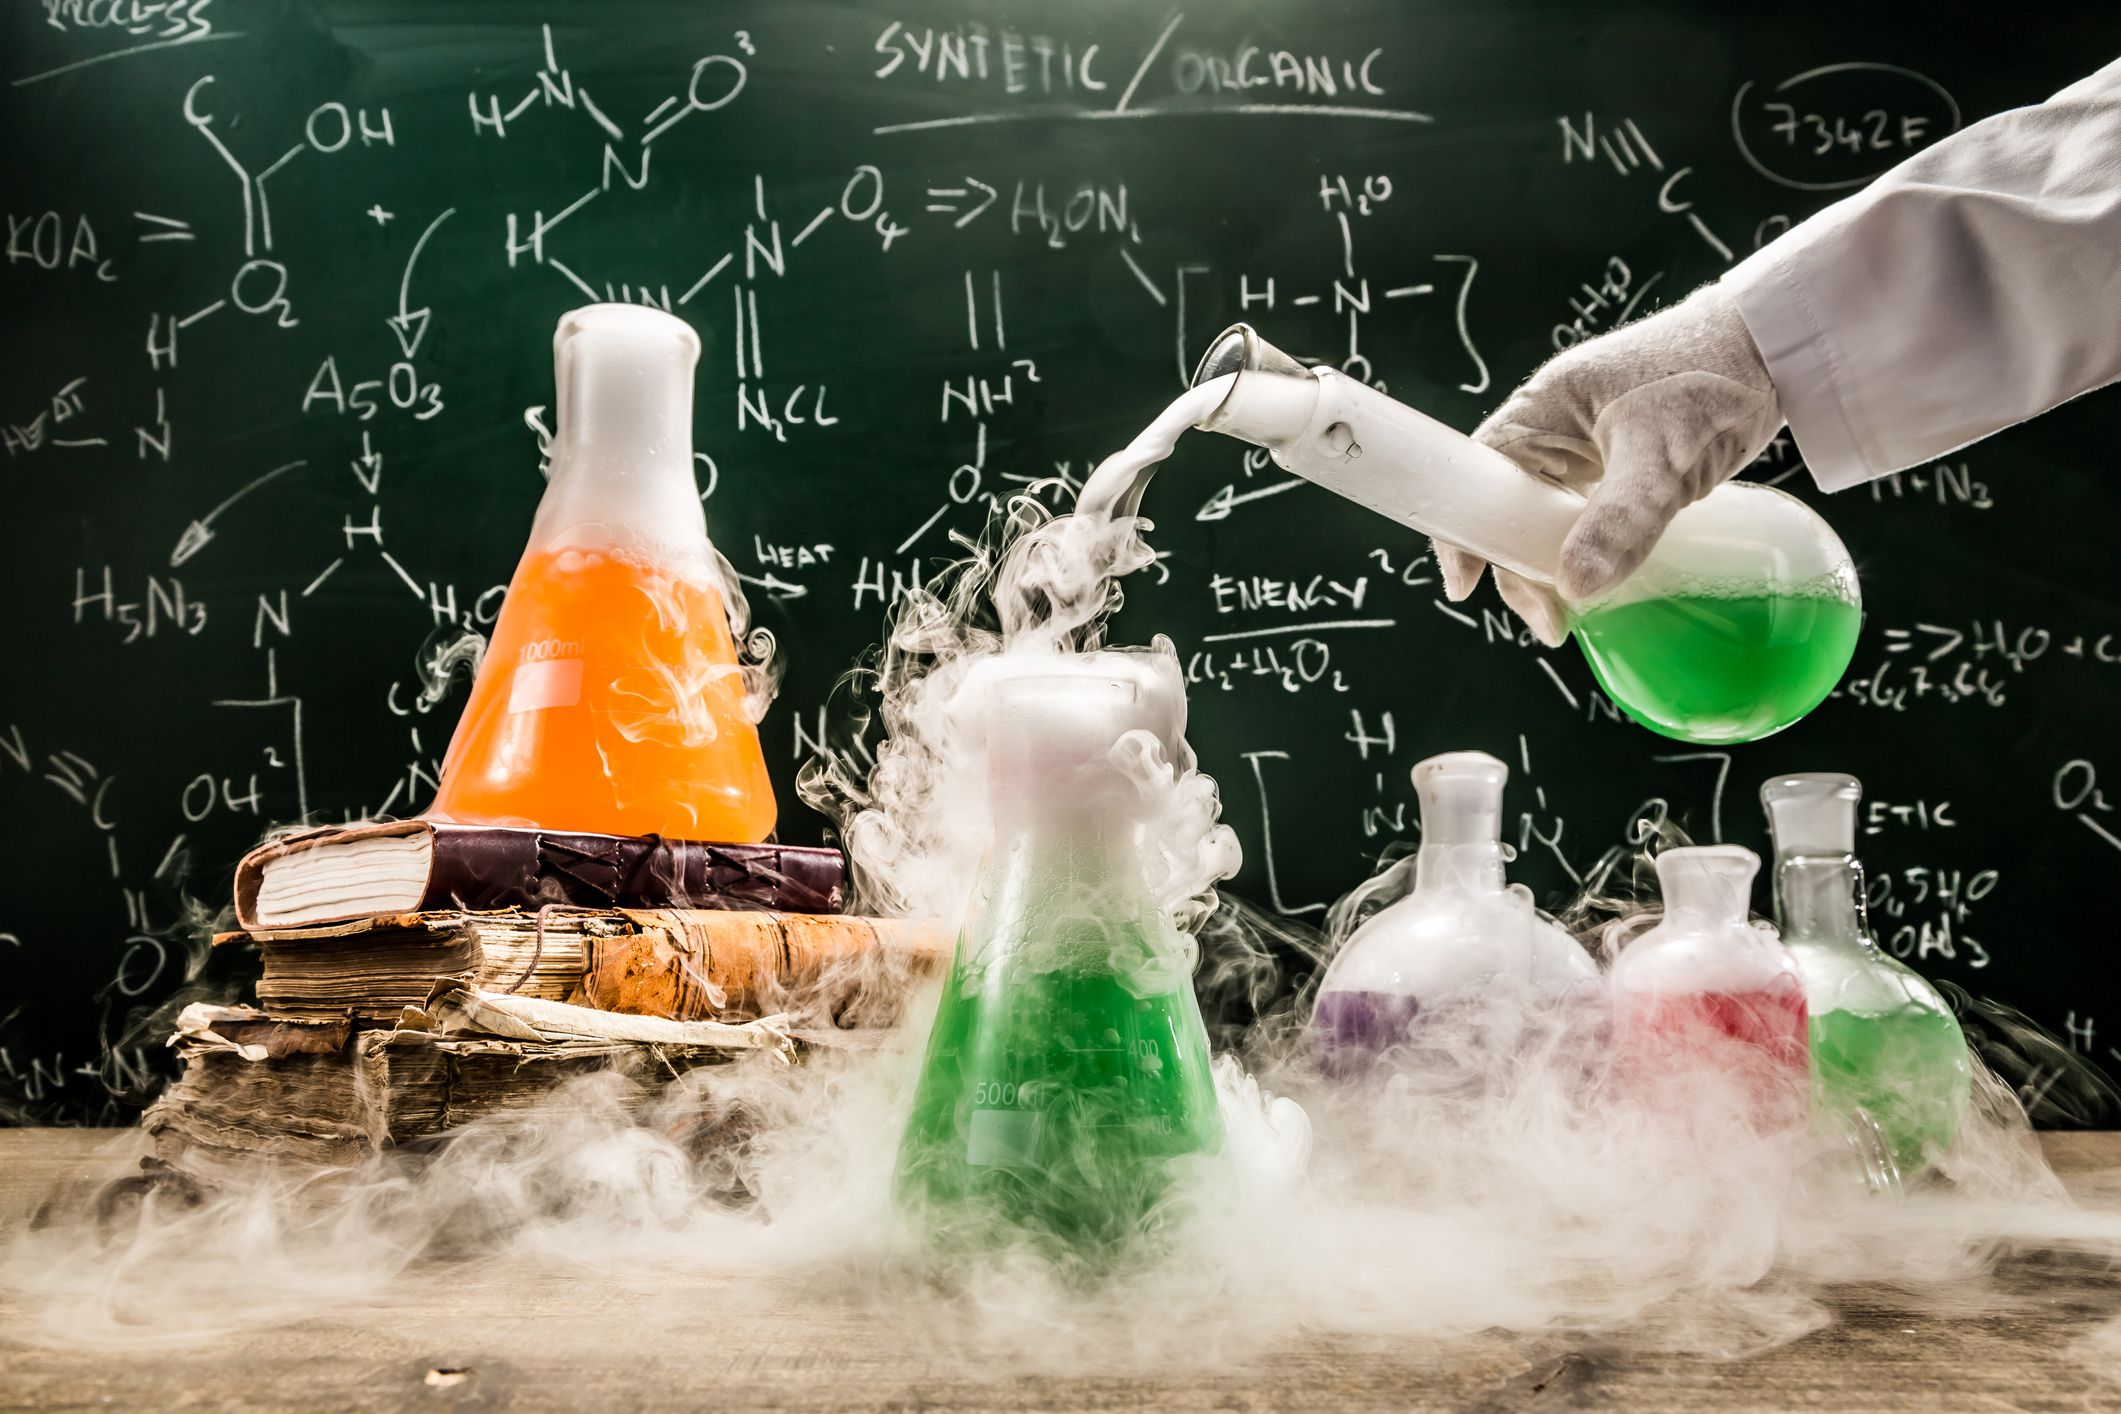
\includegraphics[width=\paperwidth,height=\paperheight]{Chemistry.jpg}
  }%
}
\usepackage{graphicx}
\graphicspath{ {./images/} }

\usepackage[pagestyles]{titlesec}
\titleformat{\chapter}[display]   
{\normalfont\huge\bfseries}{\chaptertitlename\ \thechapter}{20pt}{\Huge}   
\titlespacing*{\chapter}{0pt}{-50pt}{40pt}
\titleformat{\chapter}[display]{\normalfont\bfseries}{}{0pt}{\Huge}
\newpagestyle{mystyle}
{\sethead[\thepage][][\chaptertitle]{}{}{\thepage}}
\pagestyle{headings}

\begin{document}


\begin{tikzpicture}[font=\sffamily,remember picture,overlay]
    \path (current page.north west) node[below right,fill={rgb:orange,0.55;yellow,2.5;pink,1.5},minimum 
    width=\paperwidth,minimum height=3cm](box){};
    
    \path (box.west) node[right=5cm,align=center] %<distance can be changed to suit
    {{\fontsize{45pt}{65pt}\color{white}\textbf{Chemistry Paper 3 Notes}}\\[2mm]
    {\fontsize{30pt}{20pt}\color{white}Grass}\\[2mm]
    {\fontsize{10pt}{10pt}\color{white}July 2022}};
    
\end{tikzpicture}

\vspace{10mm}

\begingroup
\let\clearpage\relax
\chapter{Intro}
\endgroup

By Grass and me. Creating the hyperef'd table of contents is pain.

\tableofcontents

\mainmatter

\newpage
\chapter{General Experiment notes}
\setcounter{page}{3}
\begin{enumerate}
    \item Always read the full instructions for the whole experiment before starting
    \item Use appropriate apparatus \(\Rightarrow\) Transfer with measuring cylinder if they ask for a certain volume of a solution (NEVER use beaker for measurement)
    \item Reading the volume of liquid: \small If meniscus curved upwards, read the volume frm the bottom of the meniscus. If it curves downwards, read it frm the top of the meniscus. \normalsize
\end{enumerate}
\chapter{Titration}
\section{Tables}
Normal Titration Table:\\[2mm]
\begin{tabular}{|c|c|c|c|}
    \hline
    Titration Number & 1 & 2 & 3 \\
    \hline
     Final Burette Reading / \( \text{cm}^3 \) &&& \\
     \hline
     Initial Burette Reading / \( \text{cm}^3 \) &&&\\
     \hline
     Volume of R / \( \text{cm}^3 \) &&&\\
     \hline
     Best Titration Results ( \checkmark ) &&&\\
     \hline
\end{tabular}\\[2mm]
Thermometric Titration Table\\[2mm] \small
\resizebox{13cm}{!}{\begin{tabular}{|c|c|c|c|c|}
    \hline
    Final Burette Reading / \( \text{cm}^3 \) & Initial Burette Reading / \( \text{cm}^3 \) & Volume of R / \( \text{cm}^3 \) & Highest Temperature / \( \text{\degree} C \) & Total Temperature Change / \( \text{\degree} C \) \\
    \hline
     0.00 & 0.00 & 0.00 & 30.0 & 0.0 \\
     \hline
     5.00 & 0.00 & 5.00 & 32.5 & +2.5\\
     \hline
     10.00 & 0.00 & 10.00 & 35.0 & +5.0\\
     \hline
     \vdots & \vdots & \vdots & \vdots & \vdots \\
     \hline
     \(F_n\) & 0.00 \(I_n\) & \(F_n:\hspace{1mm}0.00\) & \( H_n\) & \(H_n:\hspace{1mm}+30.0\)\\
     \hline
\end{tabular}
}\\[5mm]
\textbf{Burette}\\[2mm]
\textbf{Note / AFI:}\\[2mm]
\begin{enumerate}
    \item Wash the filter funnel with the solution to be placed in the burette 
    \item Place the filter funnel on the mouth of the burette when filling it up
    \item Remove the filter funnel after, and for all burette readings
    \item Make sure the rubber tubing is filled with the solution. i.e. Ensure the tip of the burette contains no air
    \item Middle of burette clip on the middle of the rubber tubing\\
    \begin{center}
    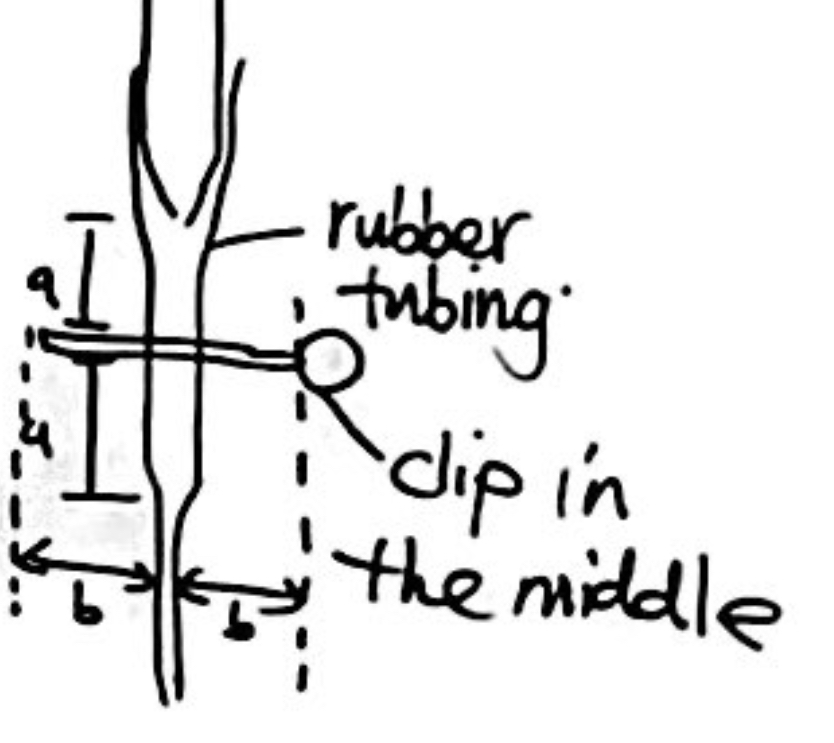
\includegraphics[scale=0.15]{images/D069C095-EBB8-4D96-A373-21AD011DD588.jpeg}
    \end{center}
    \item Burette Readings in 2 d.p.!
    \item Burette must be staightened
    \item Can use formula to calculate concentration of acid A o/r base B:\\
    Let 1 be acid A, 2 be base B
    \begin{align*}
        \frac{M_1 V_1}{n_1} &= \frac{M_2 V_2}{n_2}\\
        M_2 &= \frac{M_1 V_1 n_2}{V_2 n_1}
    \end{align*}
    Where \(M_i\) is the molar concentration of \(i\), \(V_i\) the volume of \(i\), and \(n_i\) the the mole ratio\\
    \footnotesize (in a reaction between the two substances) \normalsize
    \item T2CA
    \begin{enumerate}
        \item T - Table: 1m
        \item 2 - 2 d.p.: 1m 
        \item C - Consistency: 1m
        \item A - Accuracy: 2m
    \end{enumerate}
\end{enumerate}
\section{Pipette}
\textbf{Note / AFI:}
\begin{enumerate}
    \item Do not purposely 'tap' remaining liquid out!
    \item Holding of pipette; Hold on to the top portion when inserting the pipette filler (NOT the bulb!)
\end{enumerate}
\section{Burette + Pipette}
\hspace{1mm} 
\begin{enumerate}
    \item If solution is spilled on the sides of the conical flask, use the deionsed water to wash it off to ensure maximum accuracy.
    \item Read the burette and pipette readings at eye level. 
    \item Ensure they are no bubbles when filling up the burette and pipette 
\end{enumerate}

\section{Accuracy of Instruments}
\begin{center}
    \begin{tabular}{c|c}
    Burette & \(\pm 0.05\) (cm\(^3\)) \\
    \hline
    Pipette & 20.00 / 25.00 cm\(^3\)\\
    \hline
    Thermometer & \(\pm 0.5\) (\degree C)\\
    \hline
    Electronic Balance & 2 d.p. (g)\\
    \hline
    Measuring Cylinder & \(\pm 0.5\) (cm\(^3\))\\
    \hline
    Stopwatch & Nearest \(s\)\\
    \hline
    Gas Syringe & Nearest cm\(^3\)\\
\end{tabular}
\end{center}
\newpage
\chapter{Dessert Qns}
\begin{enumerate}
    \item A student repeated the experiment and accidentally used a 20.0cm\(^3\) pipette to measure solution \(Q\) into the flask in each titration.\\
    The student thought he had used a 25.0cm\(^3\) pipette\\
    Describe and explain the effect that this would have on the percentage by mass of iodine in the solution calculated by the student.\\[2mm]
    \(Ans:\) \underline Using 20.0cm\(^3\) of \(Q\) instead of 25.0cm\(^3\) will result in lower volume of \(R\) needed [1]. This will result in a lower concentration of \(I_2\) calculated in \(Q\) and hence a lower percentage by mass of \(I_2\) in \(Q\). [1]
    \item Explain why it is necessary to stir the mixture in the beaker before measuring the highest temperature reached by the mixture.\\[2mm]
    \(Ans:\) It is to ensure that all the metal carbonate \(X\) has reacted completely with the respective acids. [1]
    \item State one \textbf{key} source of error in the results obtained in Experiments 1 to 3 (temperature experiment). Suggest \textbf{one} improvement you could make to the experiment to reduce this error.\footnote{Experimental Error, NOT human error}\\[2mm]
    \(Ans:\) Beaker can be insulated with poor heat conductor / cover with lid nested in beaker [2]
\end{enumerate}
\newpage
\chapter{Temperature Related\\ Experiments}
\begin{enumerate}
    \item Change in temperature / enthalpy must have "+" and "-" signs
\end{enumerate}
\chapter{Q.A. Test}
\section{Note / AFI:}
\begin{enumerate}
    \item Always rmb to use test tube or Q.A. test \small -- The question might not explicitly state this \normalsize
    \item Hold boiling tube at an angle and reduce the flame height
    \item Open the bunsen burner air hole halfway \small if you have problems lighting it \normalsize
    \item Adding excess bench reagent \( \Rightarrow \) Pour some test sample away and continue adding the reagent \small (if the test tube is getting too full) \normalsize
    \item Collect solid samples with spatula \small (always use the small scoop) \normalsize
    \item Even if there is nothing seen/heard/smelled for a particular step, the observation should still be written, as "No visible Change".
    \item When writing observations rmb to put \textbf{all} the information down. \footnote{E.g.: What is the color and smell of the gas; write colorless and odorless if nothing specific seen or smelled} \normalsize
    \item Some observations required are implied, but not explicitly stated. \footnote{E.g.: Place the boiling tube in the test-tube rack to allow its contents to settle.\\
    \( \Rightarrow \) After waiting, rmb to add in the observation for this; like "Blue precipitate settled at the bottom of the test tube.}
\end{enumerate} \vspace{2mm}
\section{Best/Modal Answers for Observations:}
\begin{enumerate}
    \item Nothing happens \(\Rightarrow\) No visible change
    \item Add aqueous ammonia slowly and stir with a glass rod until no further changes are seen \(\Rightarrow\) \footnote{No need write in the front like: "Upon adding aqueous ammonia / silver nitrate / whatever reagents"}A light blue precipitate was formed, which dissolved in excess to form a deep blue solution
\end{enumerate}

\newpage

\chapter{Experimental Planning}
\section{Things to have}\small 
(in order which they should be presented)
\begin{enumerate}
    \item Diagram 
    \item Approach: \small (Short summary of what the experiment is going to be)\footnote{E.g.: \scriptsize \begin{enumerate}
        \item Approach: Comparing the effectiveness of the 3 metal oxide catalysts by measuring the volume of oxygen produced after a fixed time 
        \item Approach: Measure mass of contents before and after heating using electronic balance
    \end{enumerate}}
    \item Steps: 1.
    \item 2.
    \item \(\vdots\)
    \item \(n.\)
    \item Conclusion \footnotesize (Look at the qns to know what to write here, i.e results that can be conculded after the expt)\footnote{E.g.:\scriptsize \begin{enumerate}
        \item The metal oxide that takes the least amount of time to produce 50cm\(^3\) of oxygen gas is the most effective catalyst, while the one that takes the longest time is the least effective catalyst.
        \item Use the formula \(\frac{\text{mass before heating}-\text{mass after heating}}{\text{mass of hydrated crystals}} \times 100 \% \) to find the percentage mass of water in copper (II) sulfate crystals
    \end{enumerate}}
\end{enumerate}
\section{Notes for Steps}
\begin{enumerate}
    \item Be specific. Don't leave it up to interpretation. i.e. Write down the mass / volume of reagent to be added.
\end{enumerate}
{\section{Apparatus Drawing}
\begin{center}
    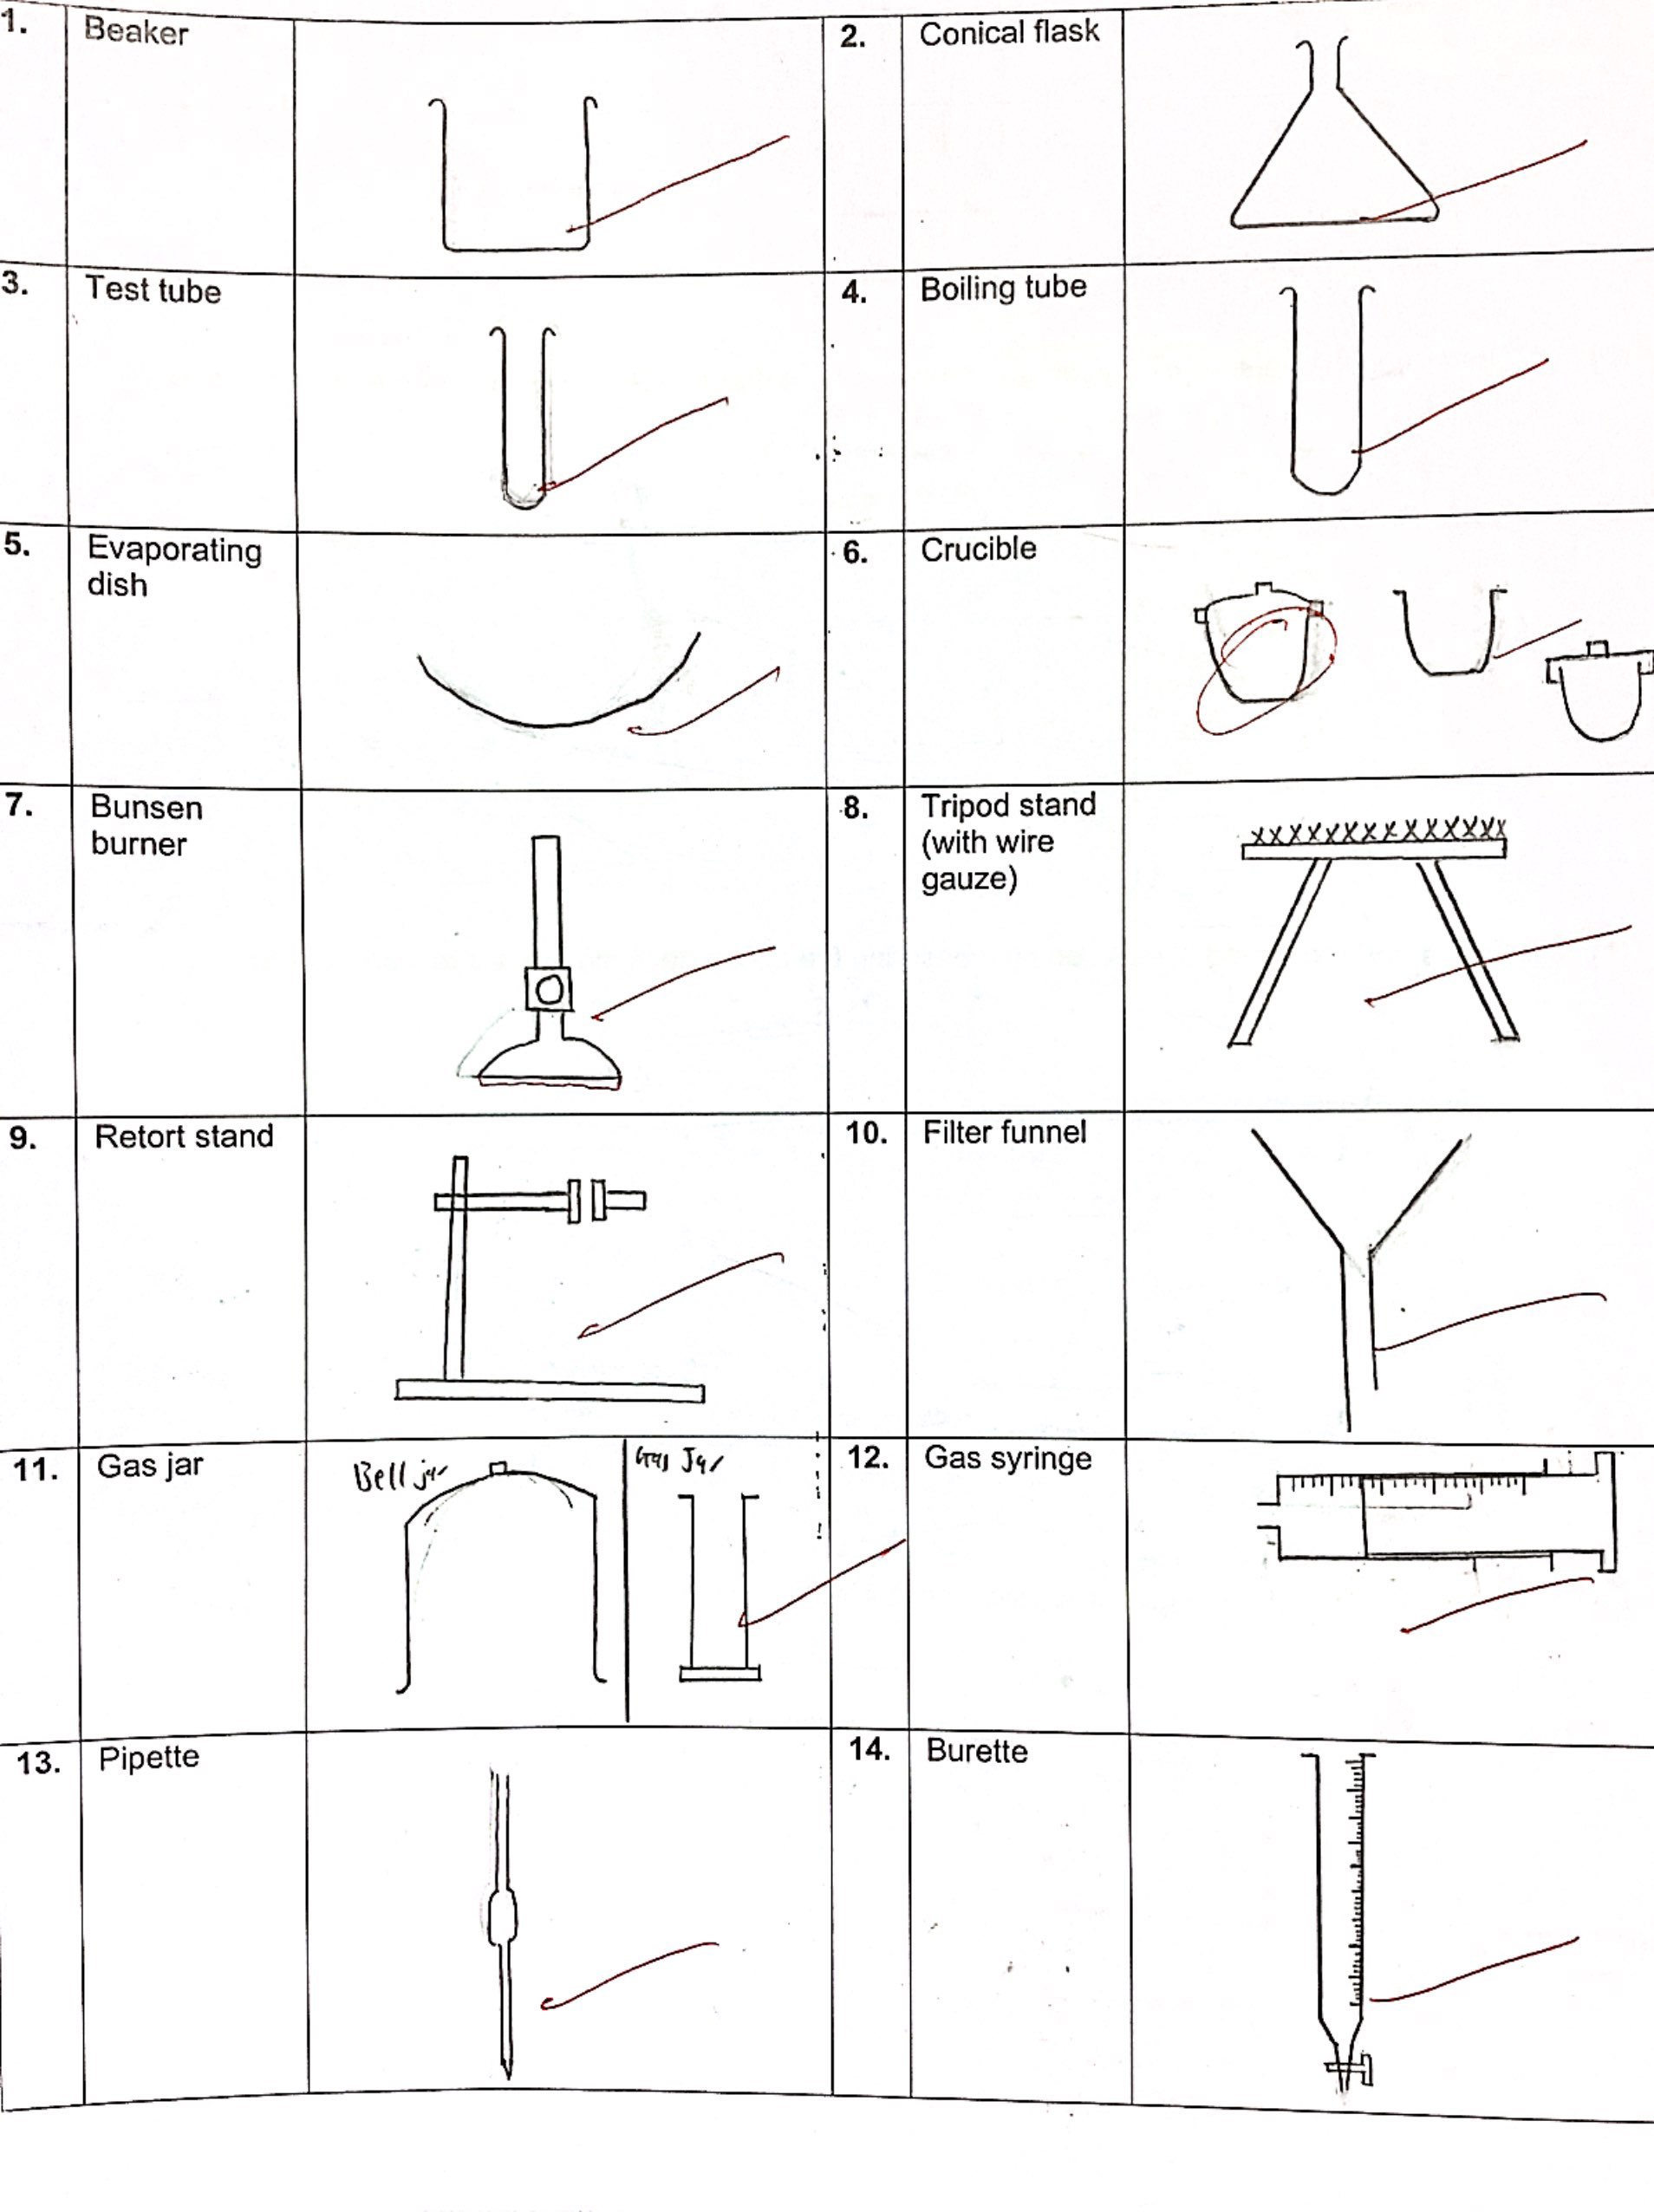
\includegraphics[width=\textwidth,height=\textheight,keepaspectratio]{images/39FFEC3F-8CED-48DC-A3E6-553D6CE7B4F8.jpeg}\\
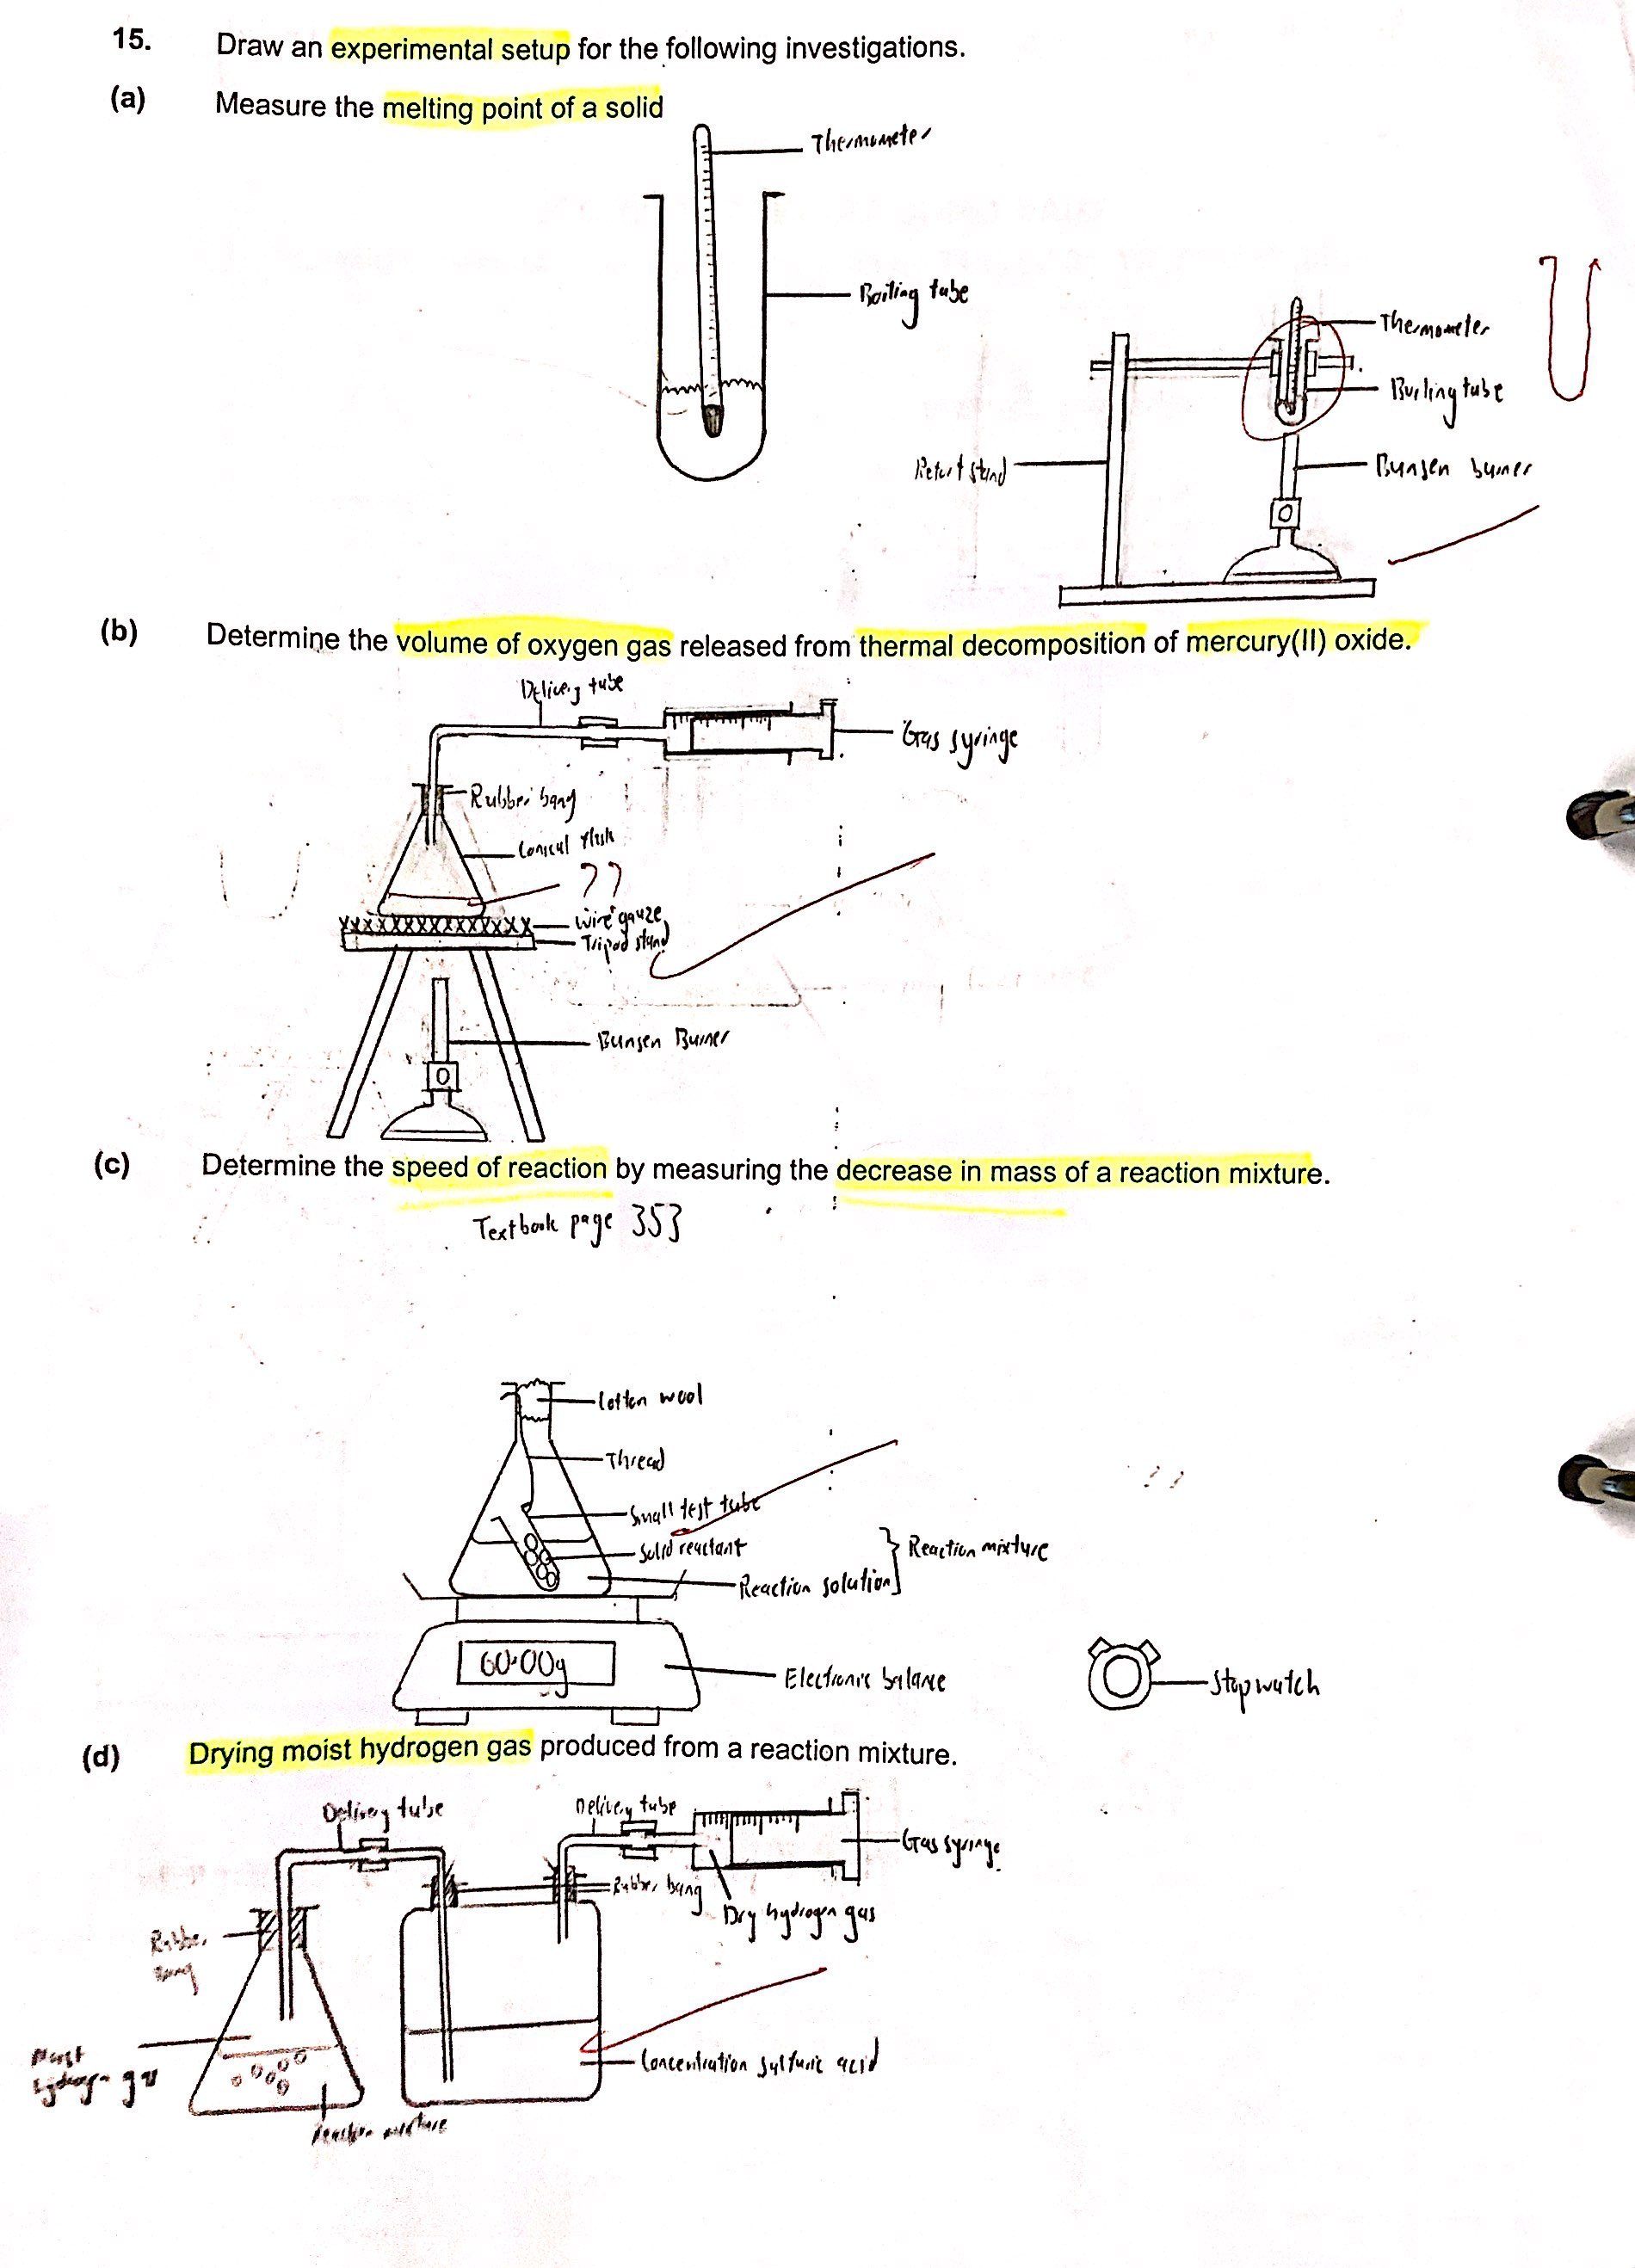
\includegraphics[width=\textwidth,height=\textheight,keepaspectratio]{images/ED948B7C-1CFB-4480-AC9D-D799496A95CE.jpeg}
\end{center}}
\chapter{Examples}
\section{Titration}
\subsection{Timed Assignment 2022: Paper 3 Practical}
\begin{center}
    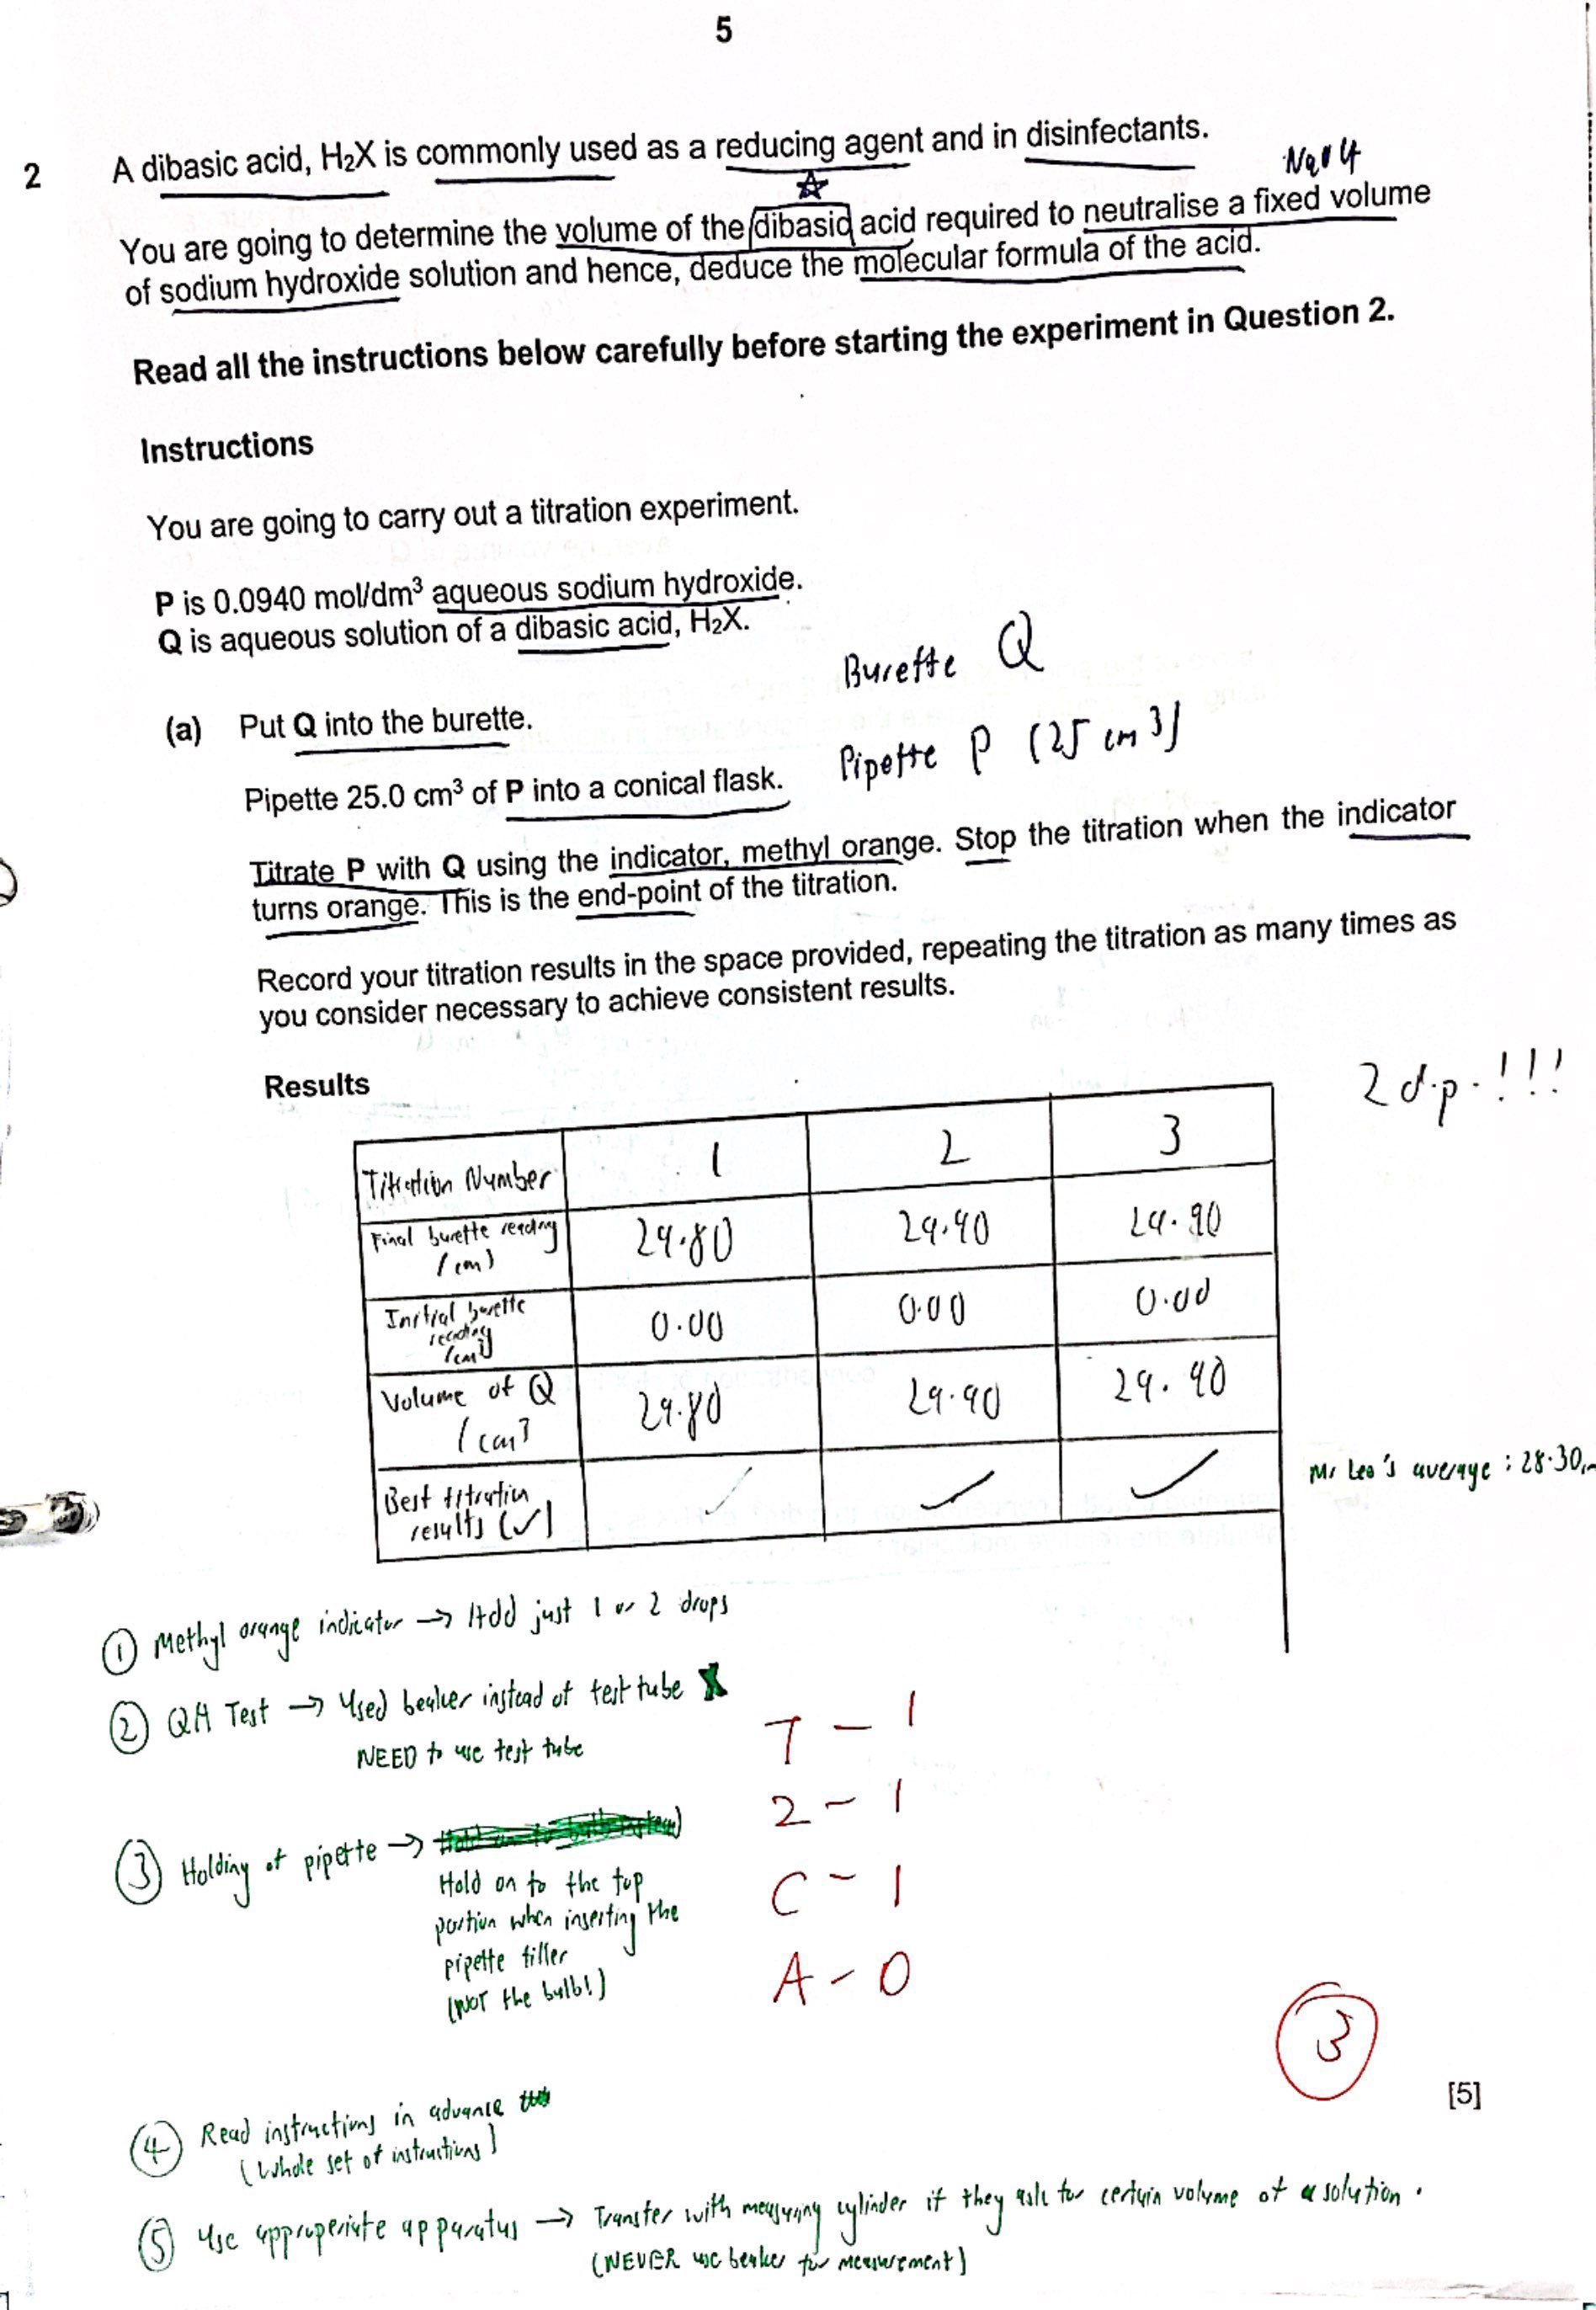
\includegraphics[scale=0.15,keepaspectratio]{images/3DFB9495-1050-41B9-849A-D6F49B74F7E5.jpeg}\\
    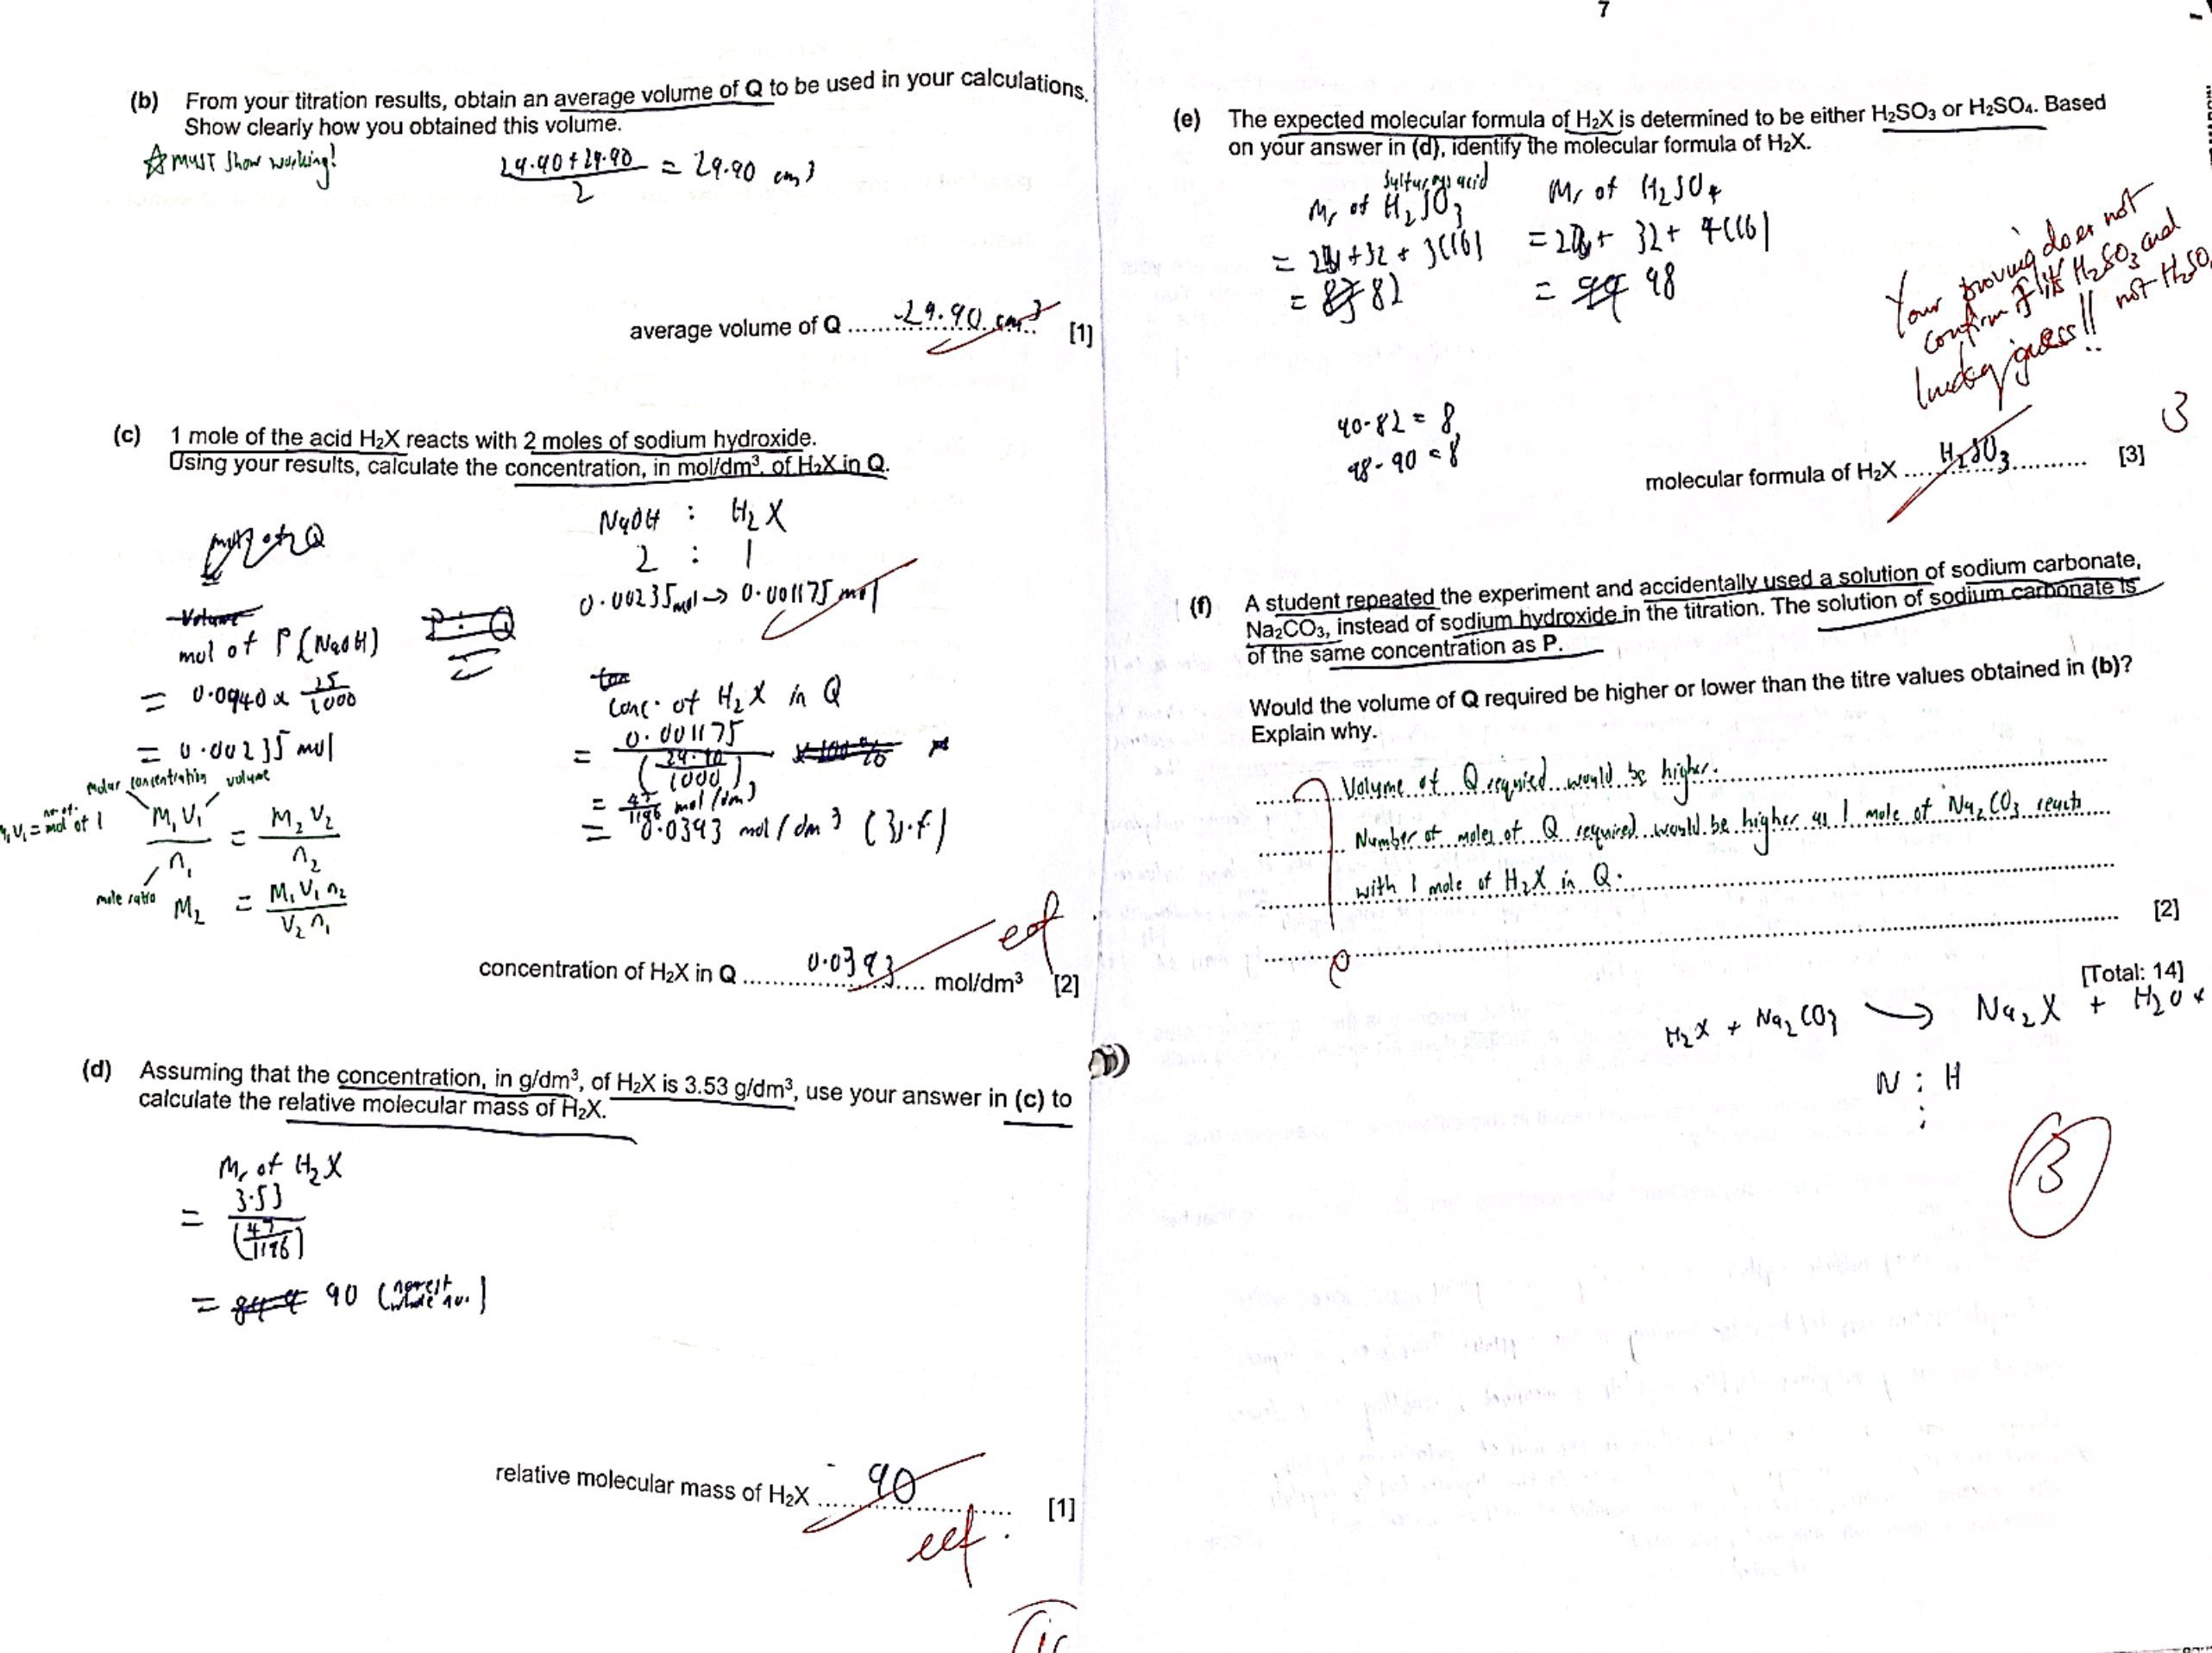
\includegraphics[width=\textwidth,height=\textheight,keepaspectratio]{images/C6D5D938-29AD-42AA-A4DB-FA04C2E56D5B.jpeg}
\end{center}
\subsection{Iodine Antiseptic }
\begin{center}
    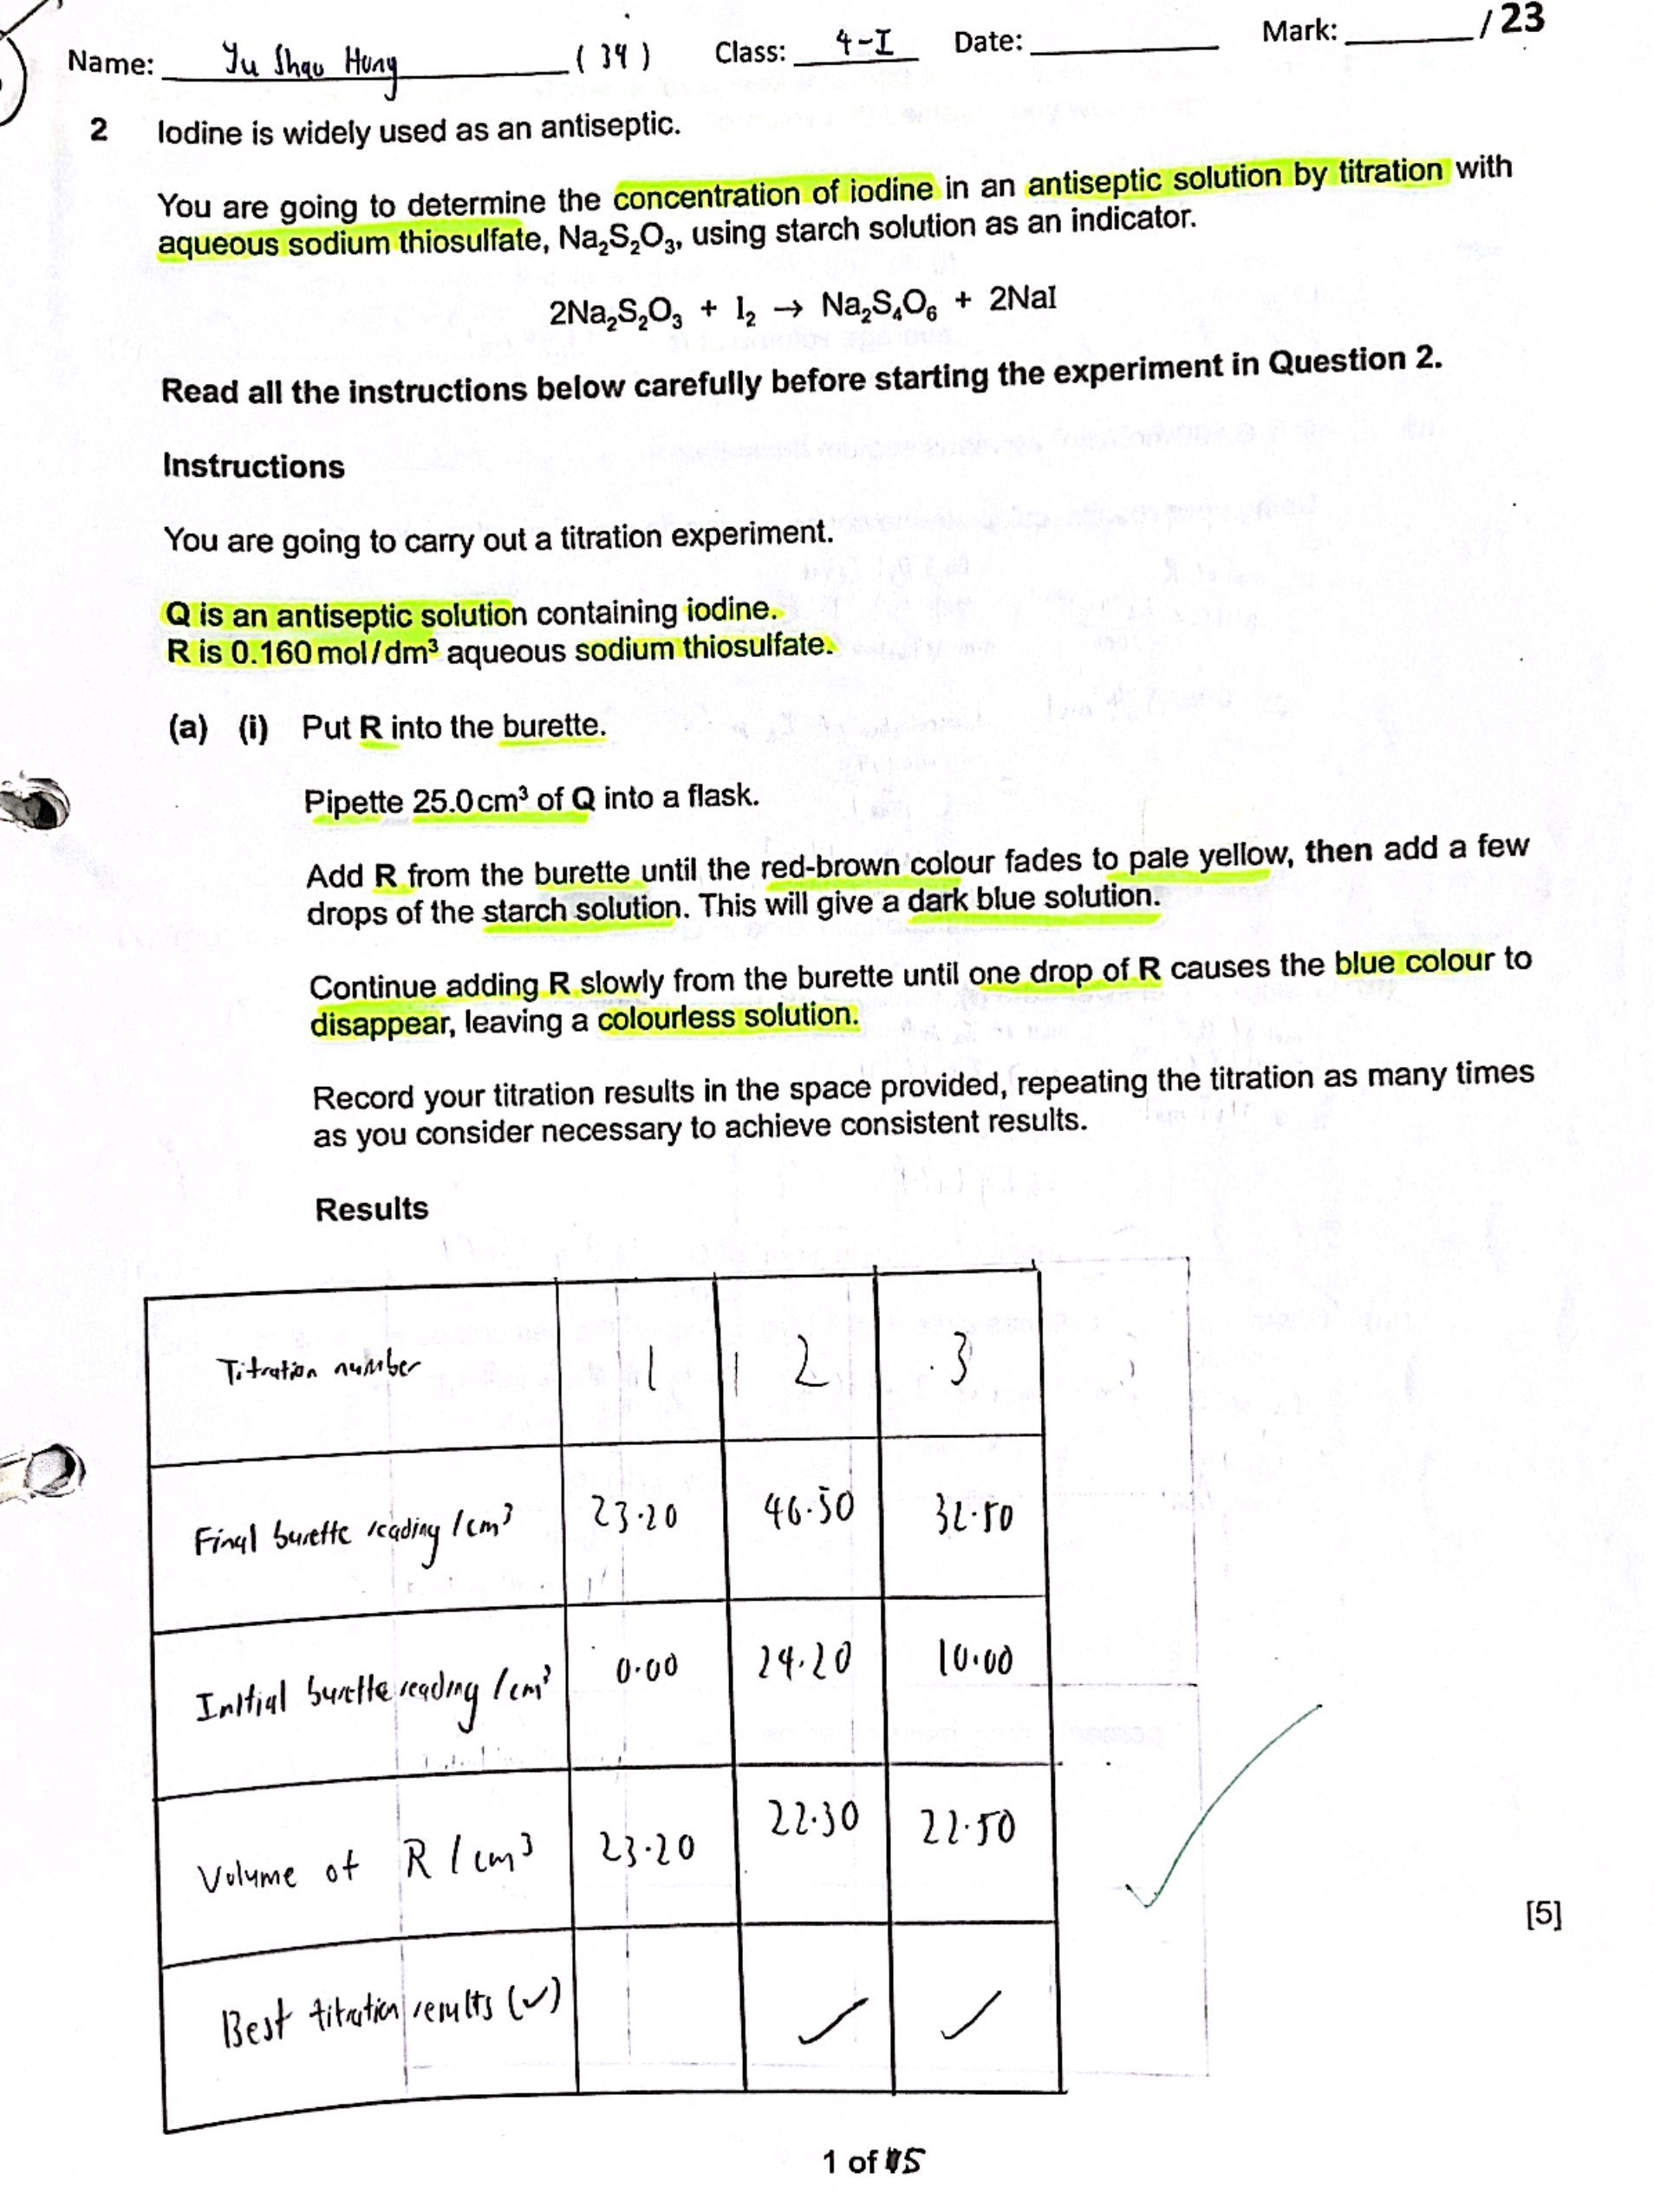
\includegraphics[width=\textwidth,height=\textheight,keepaspectratio]{images/3485CD0D-0FC4-454A-921C-FCD39763EFCE.jpeg}\\
        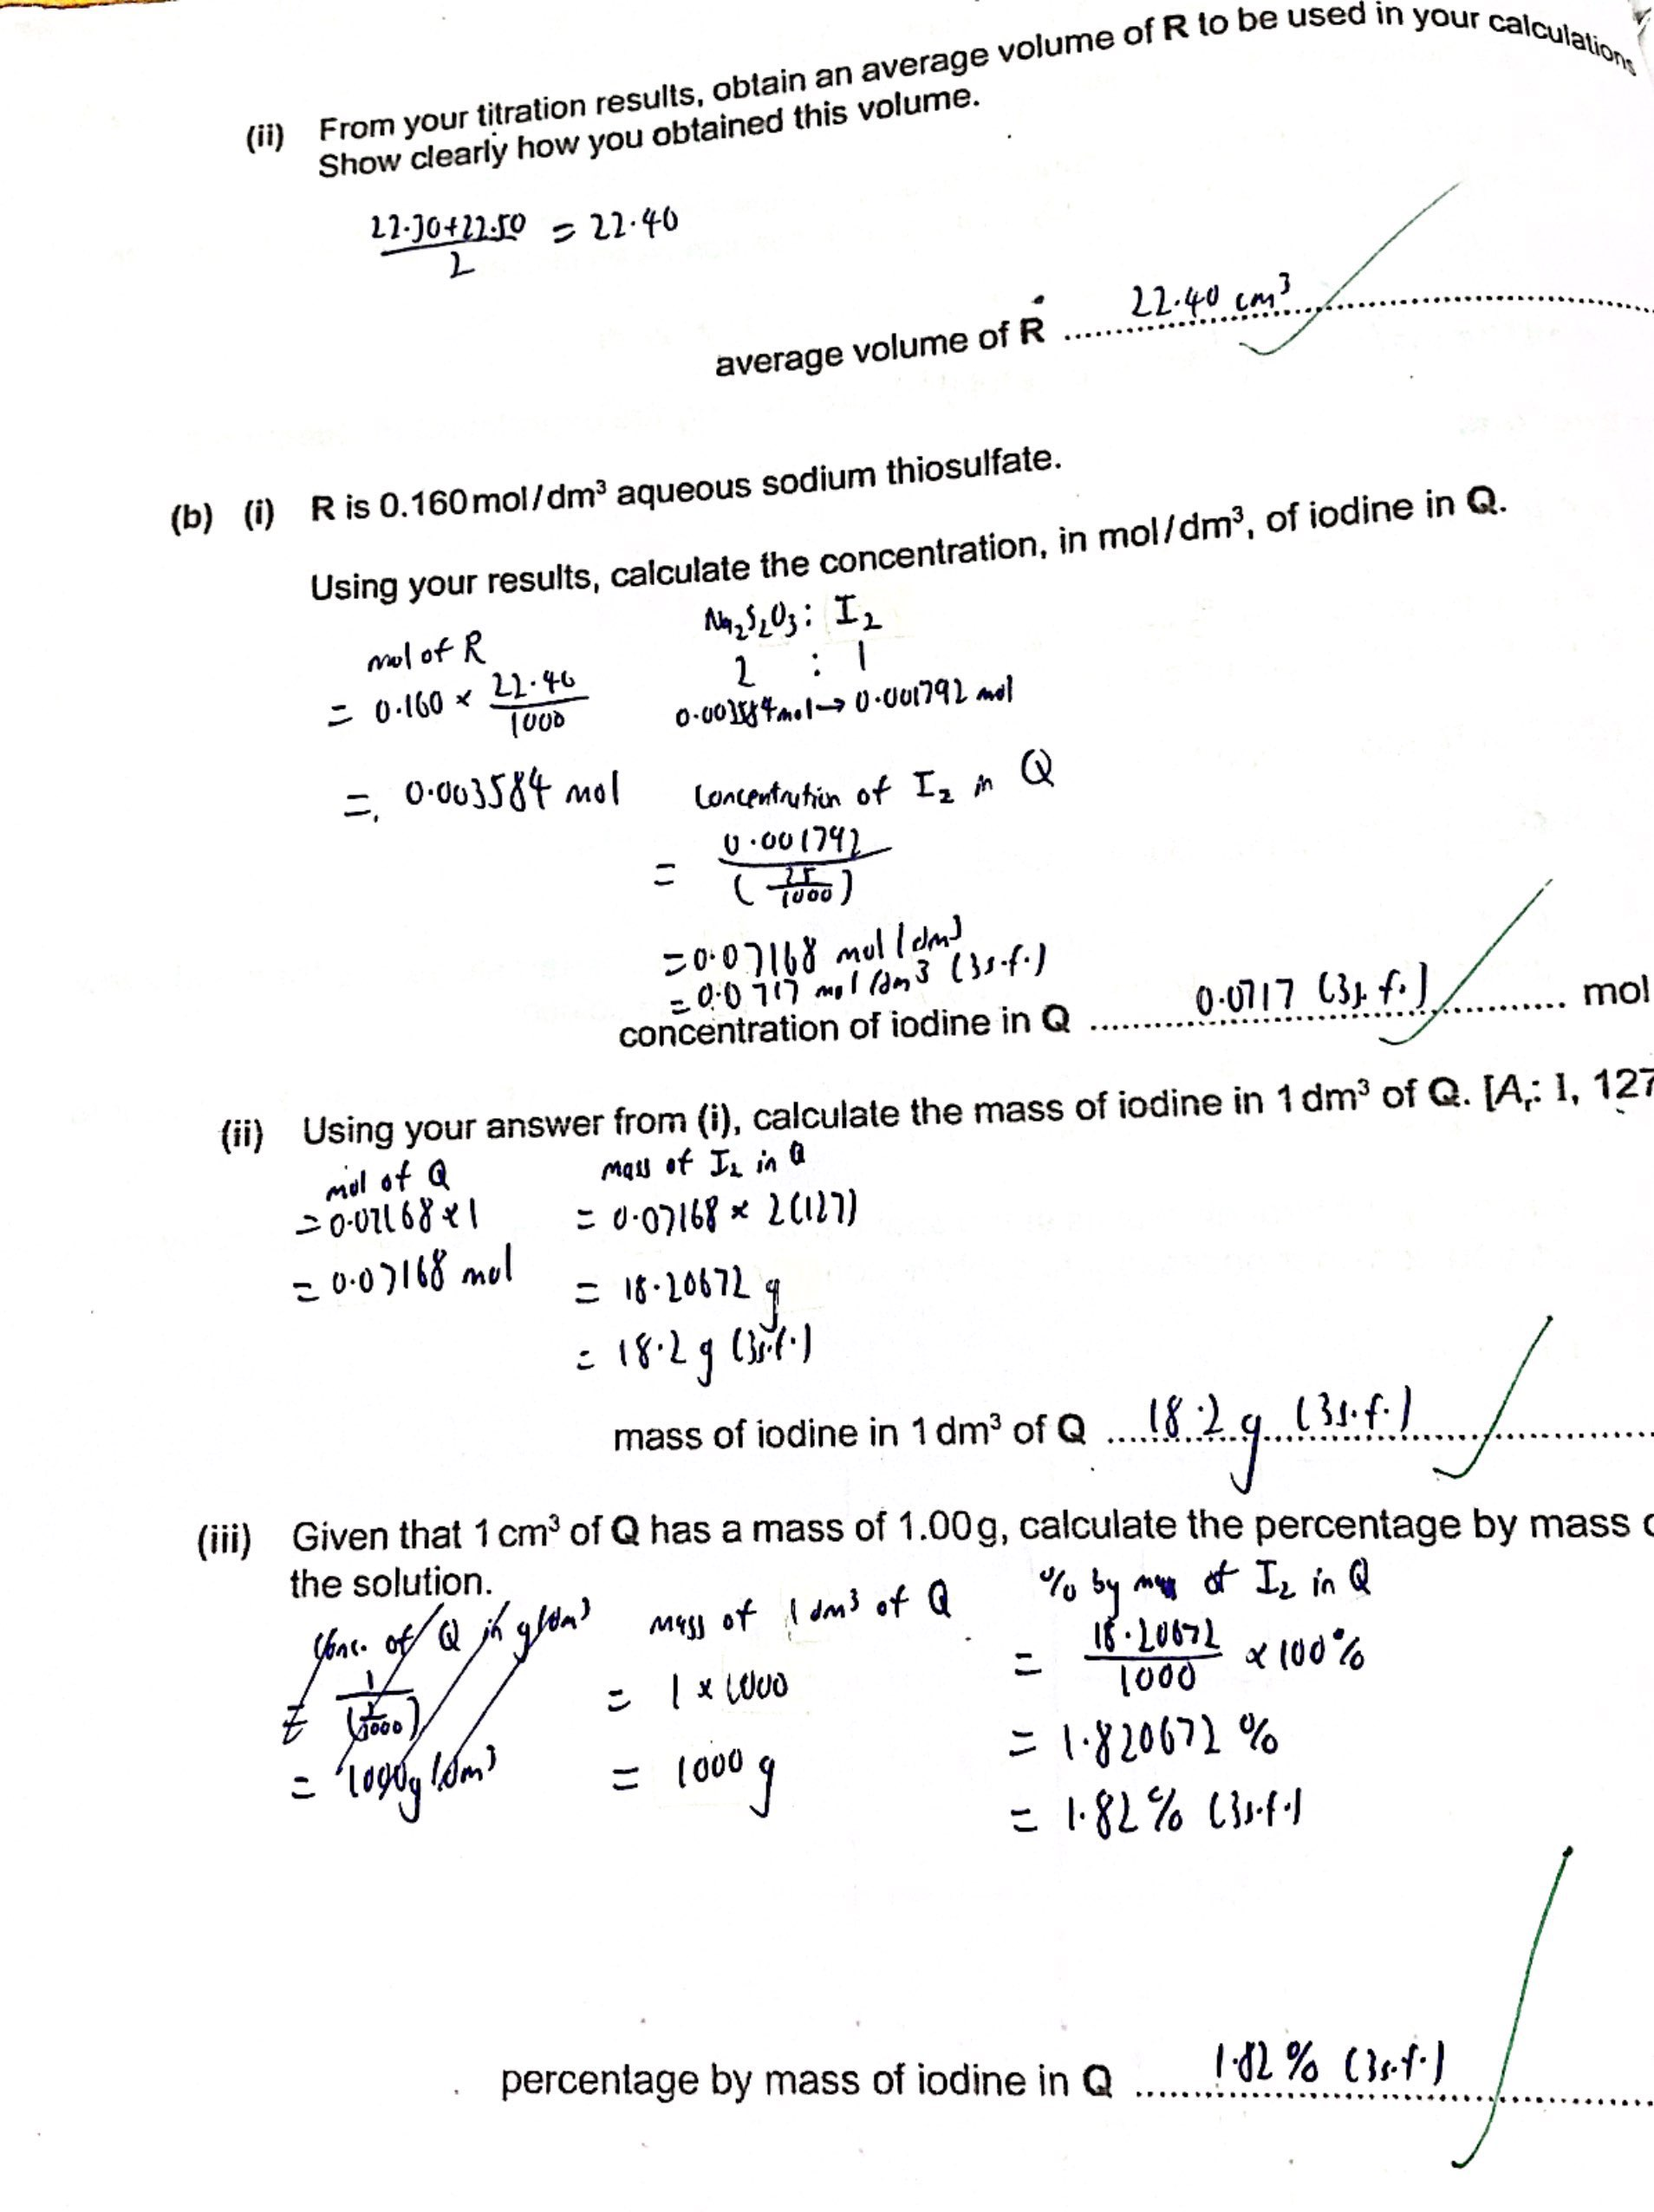
\includegraphics[width=\textwidth,height=\textheight,keepaspectratio]{images/D9D56D6E-4EA3-42B8-B9DC-6B69A7EDA7AE.jpeg}\\
        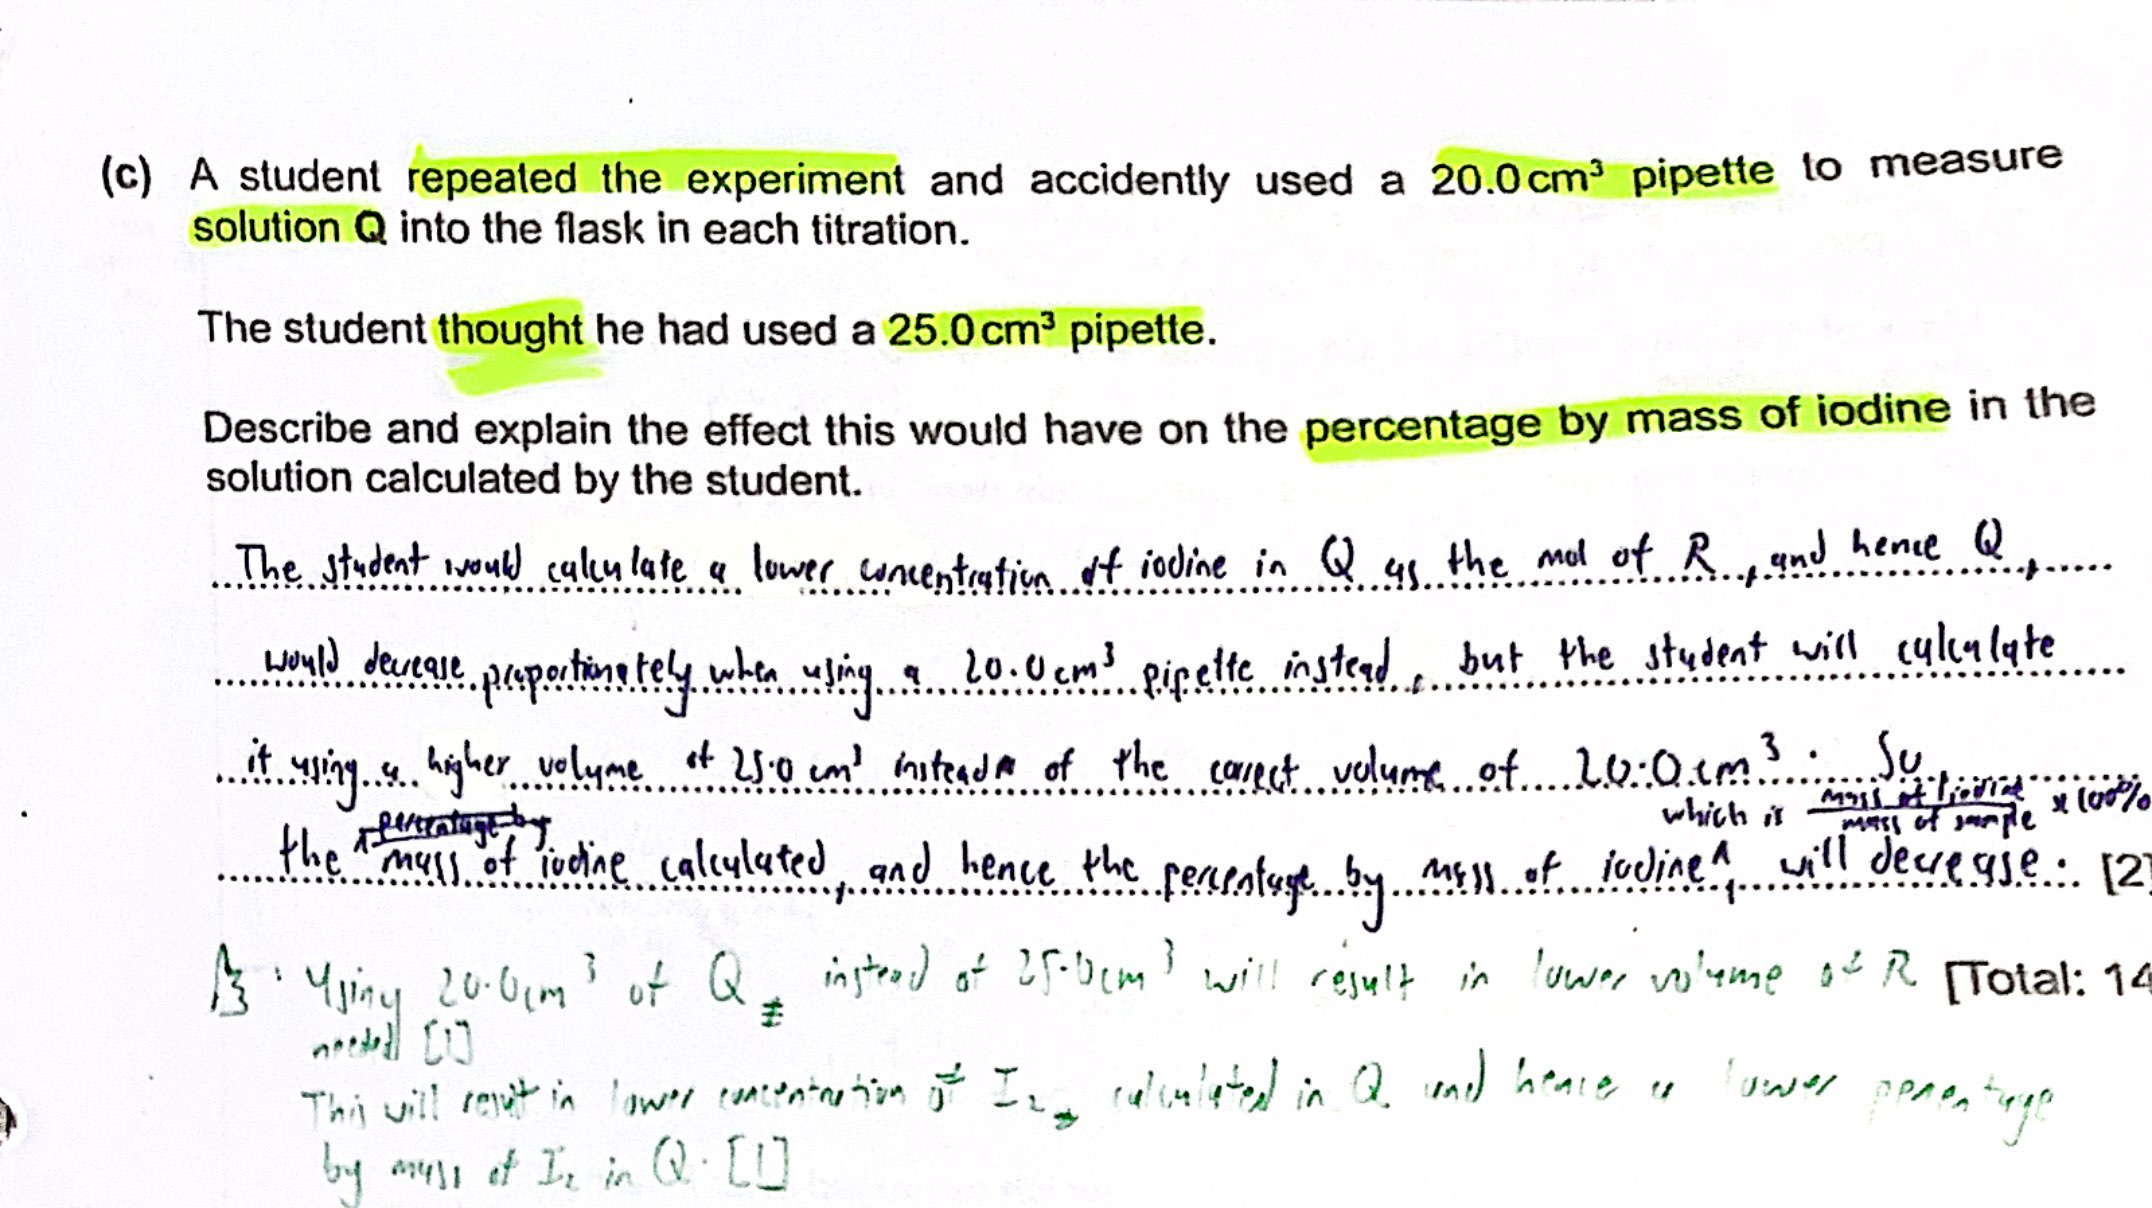
\includegraphics[width=\textwidth,height=\textheight,keepaspectratio]{images/F7022429-B8B7-402E-A2D4-0BDFD17A3484.jpeg}
\end{center}
\newpage
\subsection{Experiment on Volumetric Analysis 4 April 2022}
\begin{center}
    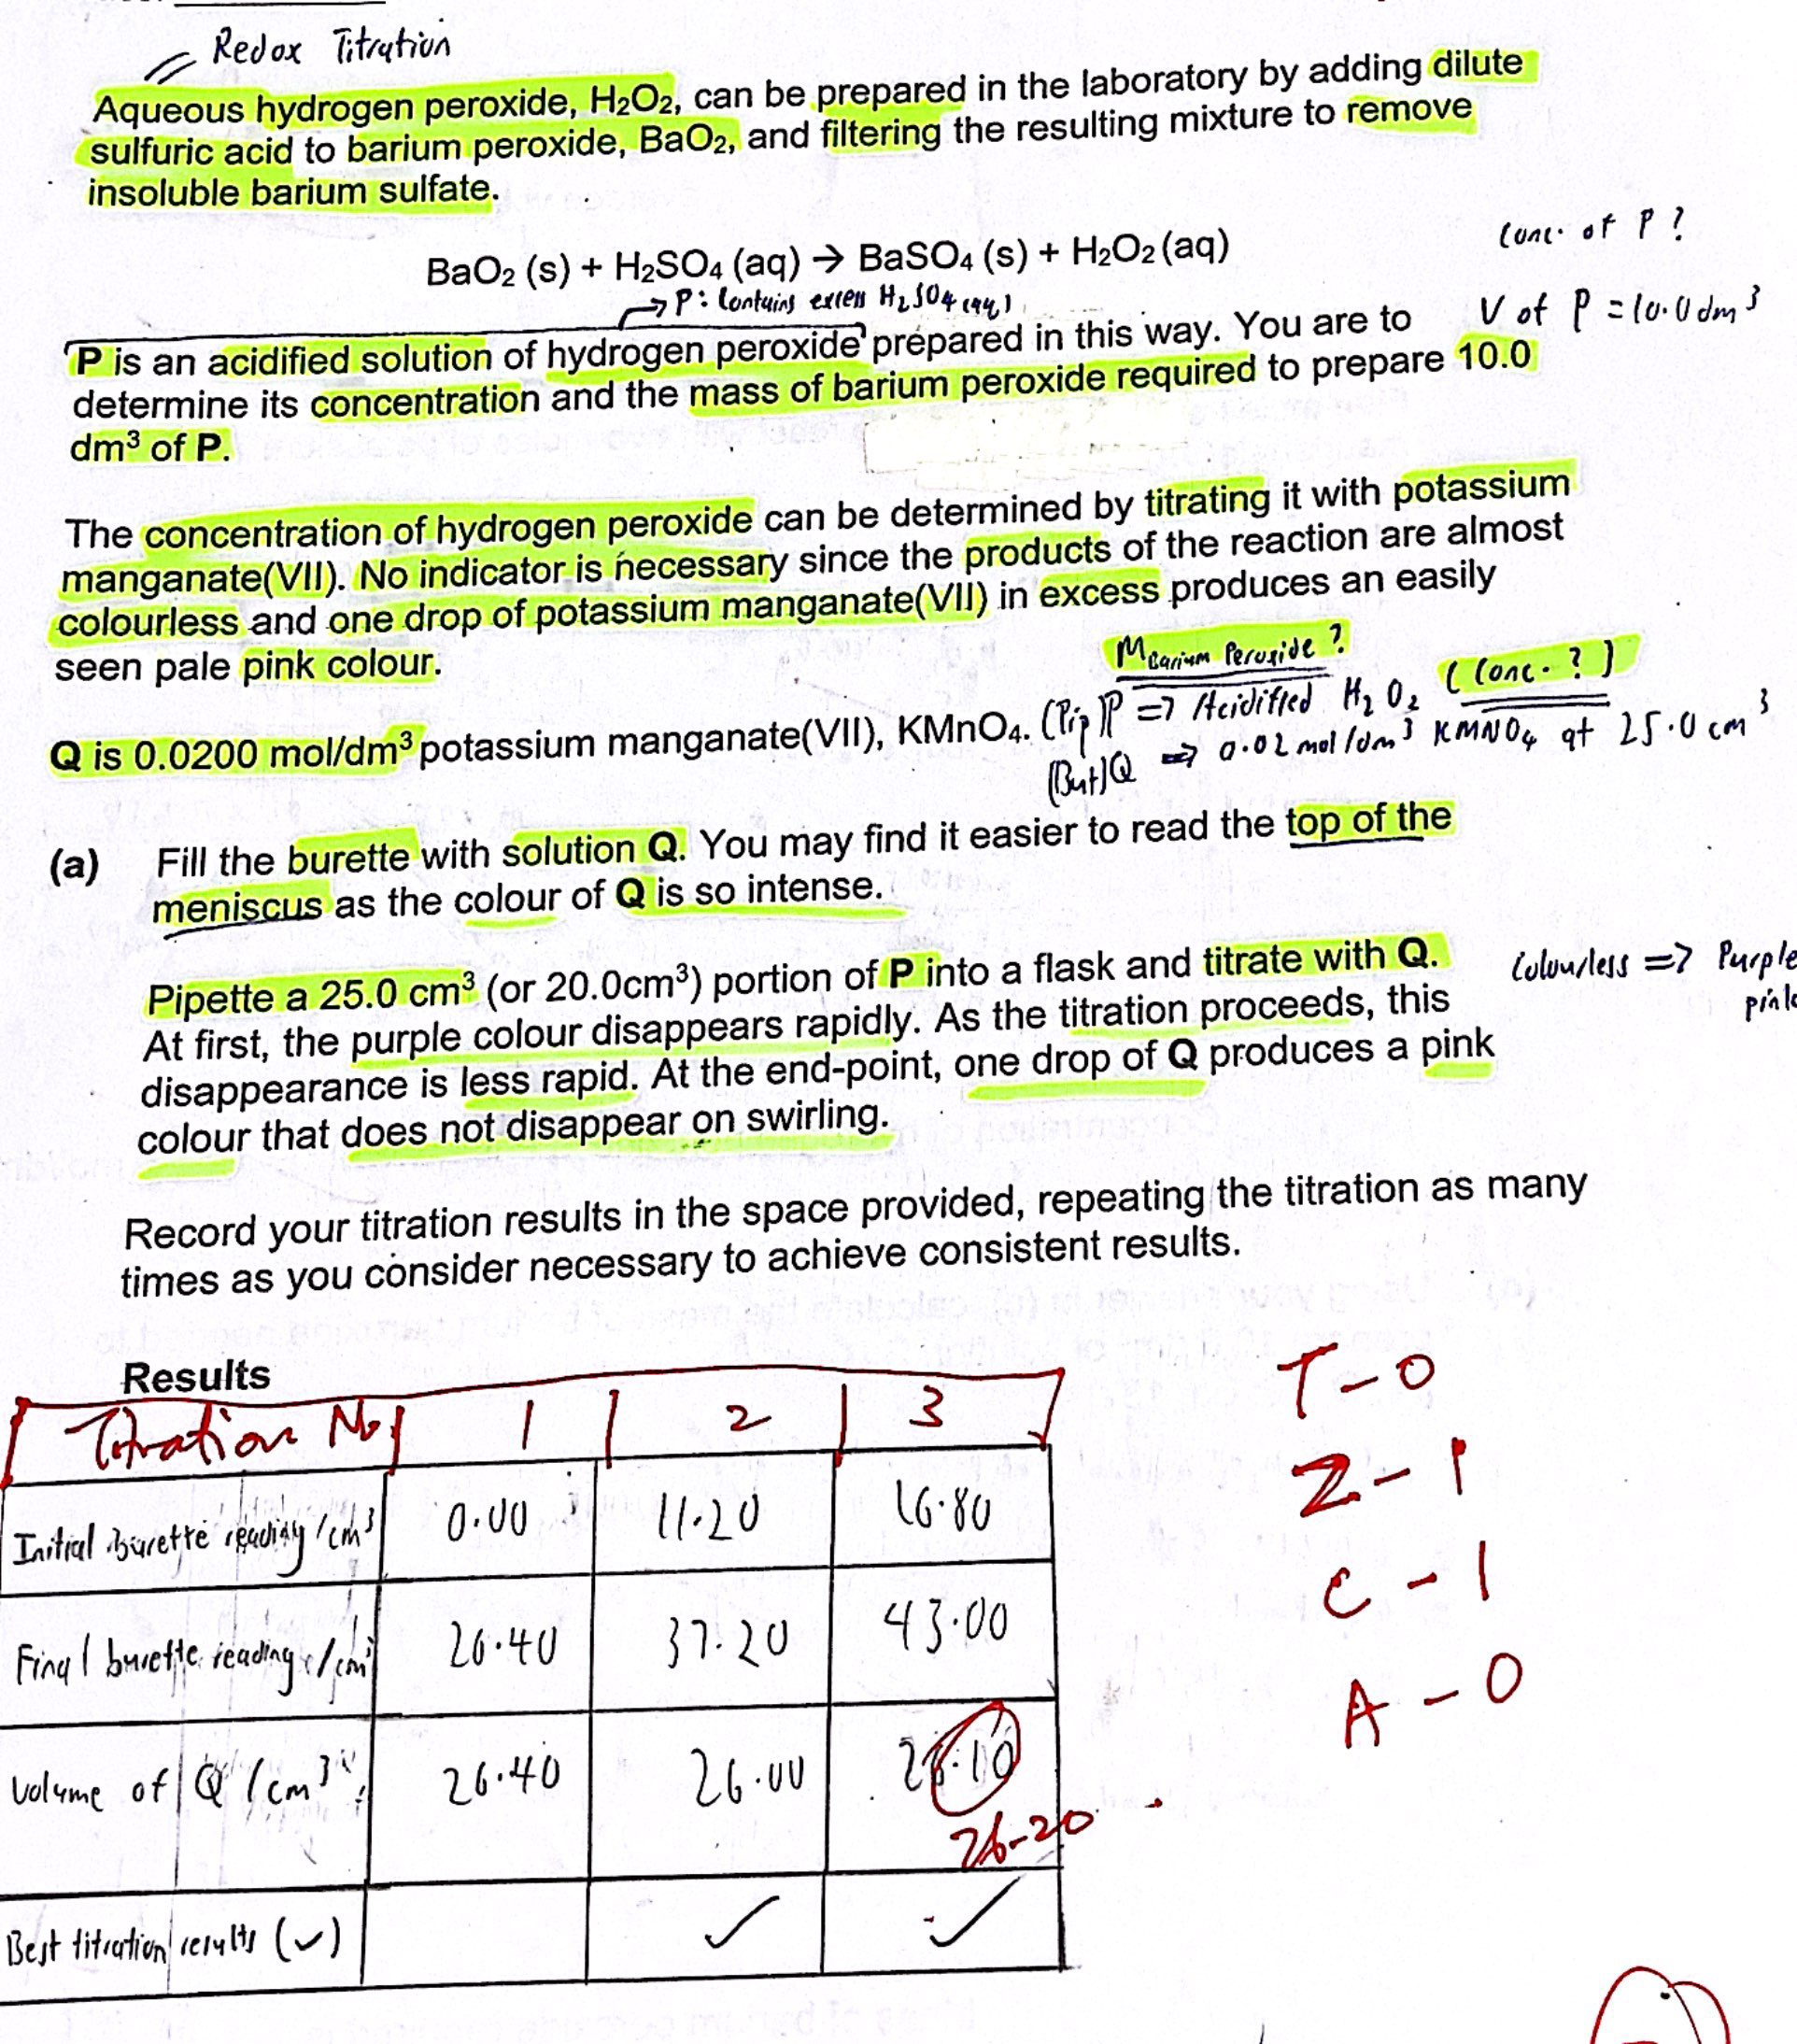
\includegraphics[width=\textwidth,height=\textheight,keepaspectratio]{images/308E24F7-4813-47C9-B60B-591E81D02F4B.jpeg}\\
        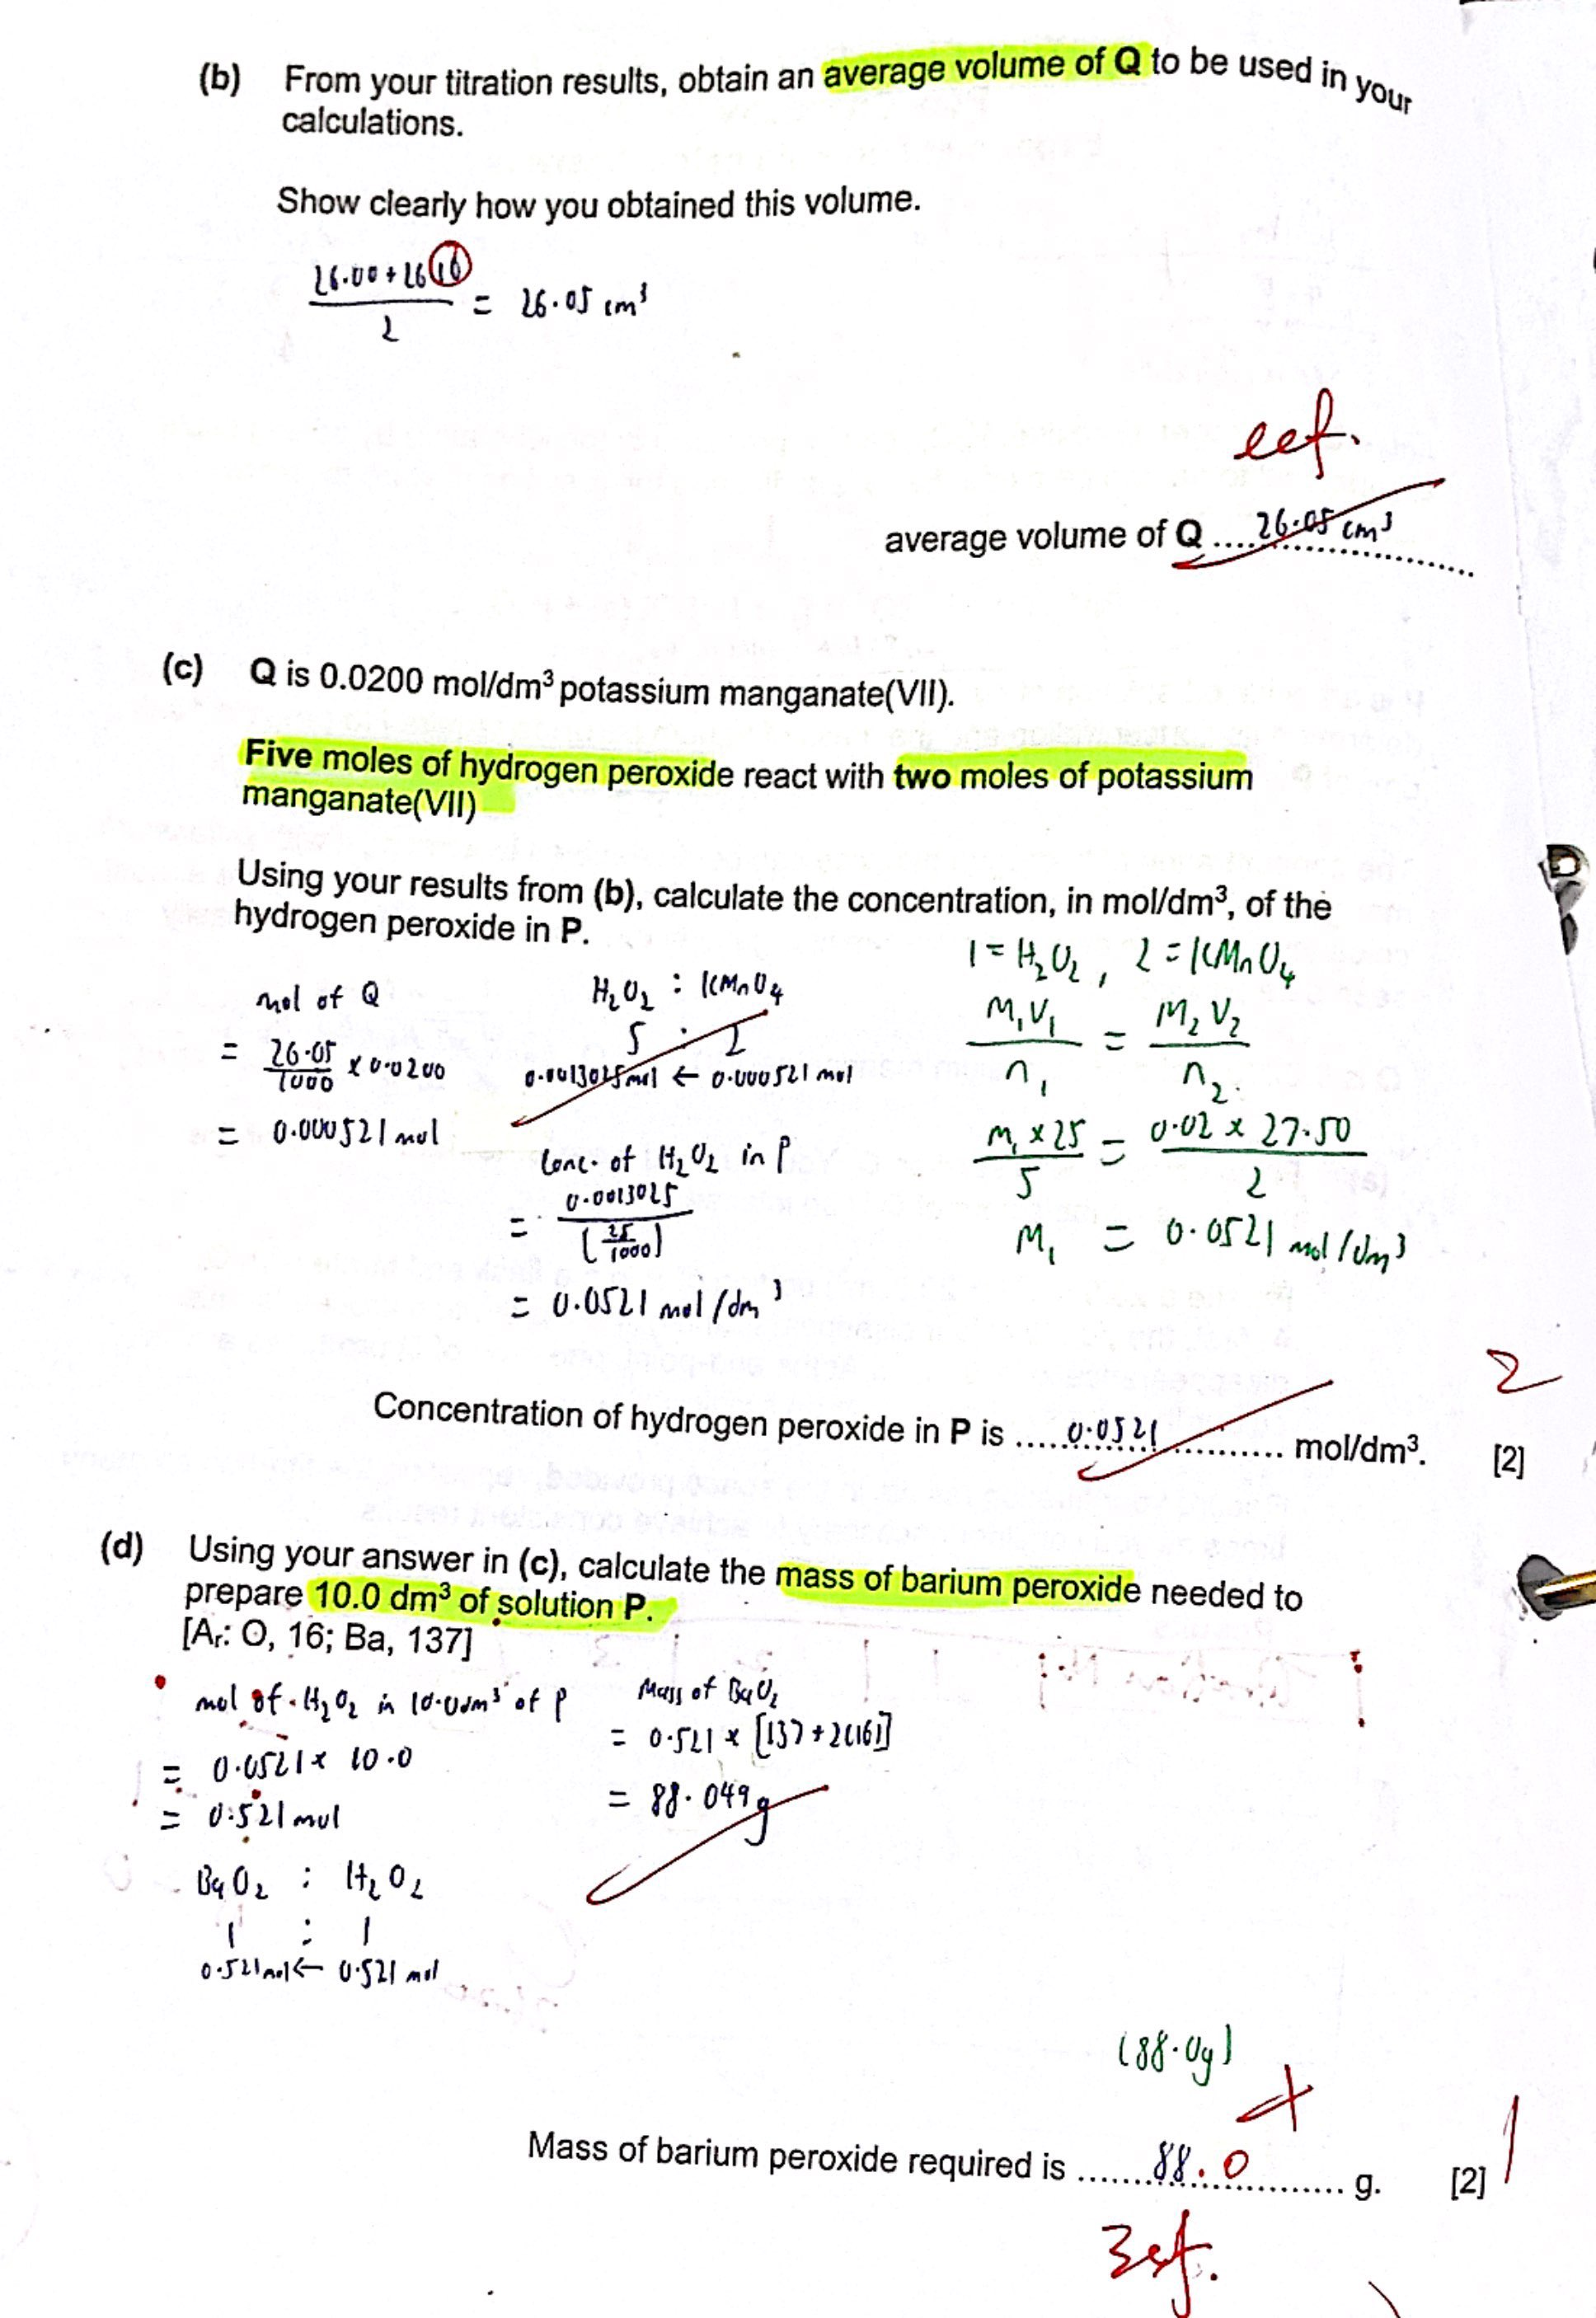
\includegraphics[width=\textwidth,height=\textheight,keepaspectratio]{images/4369A5A1-83B5-4492-8347-CC184A675AD3.jpeg}
\end{center}
\newpage
\section{Short Experiment}
    \subsection{Timed Assignment 2022: Paper 3 Practical} \begin{center}
        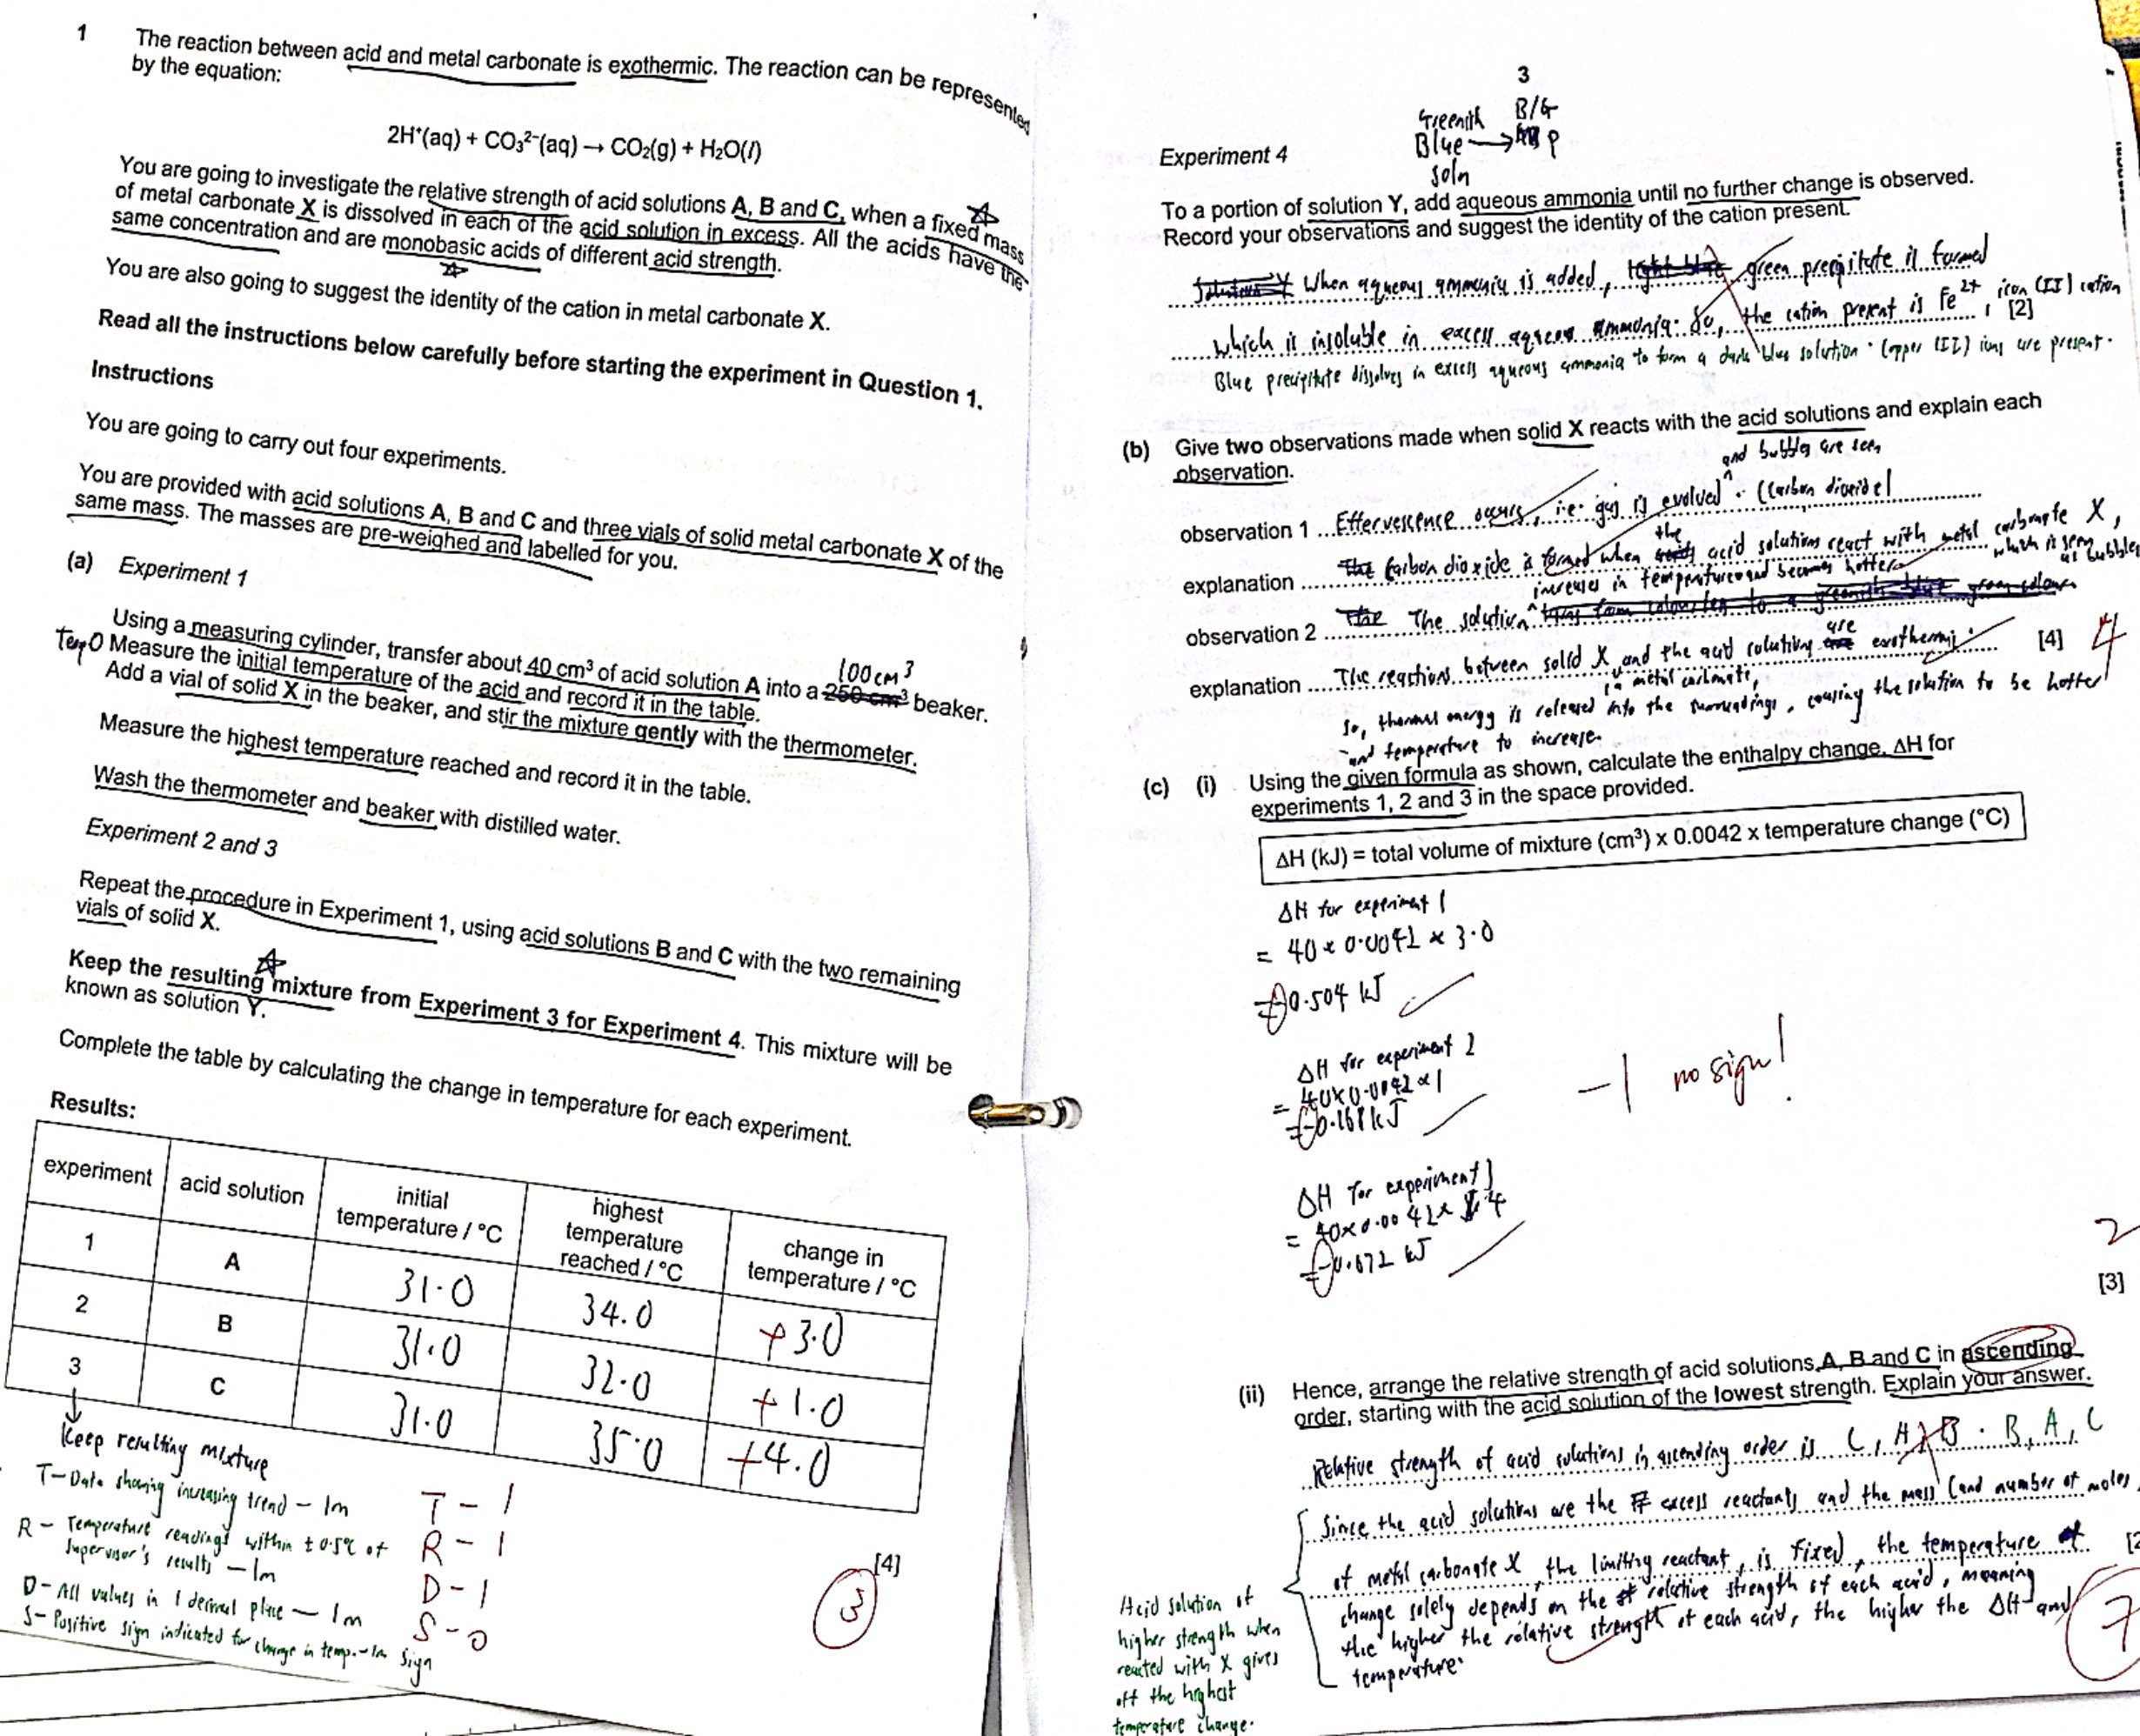
\includegraphics[width=\textwidth,height=\textheight,keepaspectratio]{images/3160BCD6-275B-4763-9466-9476828388DA.jpeg}\\
        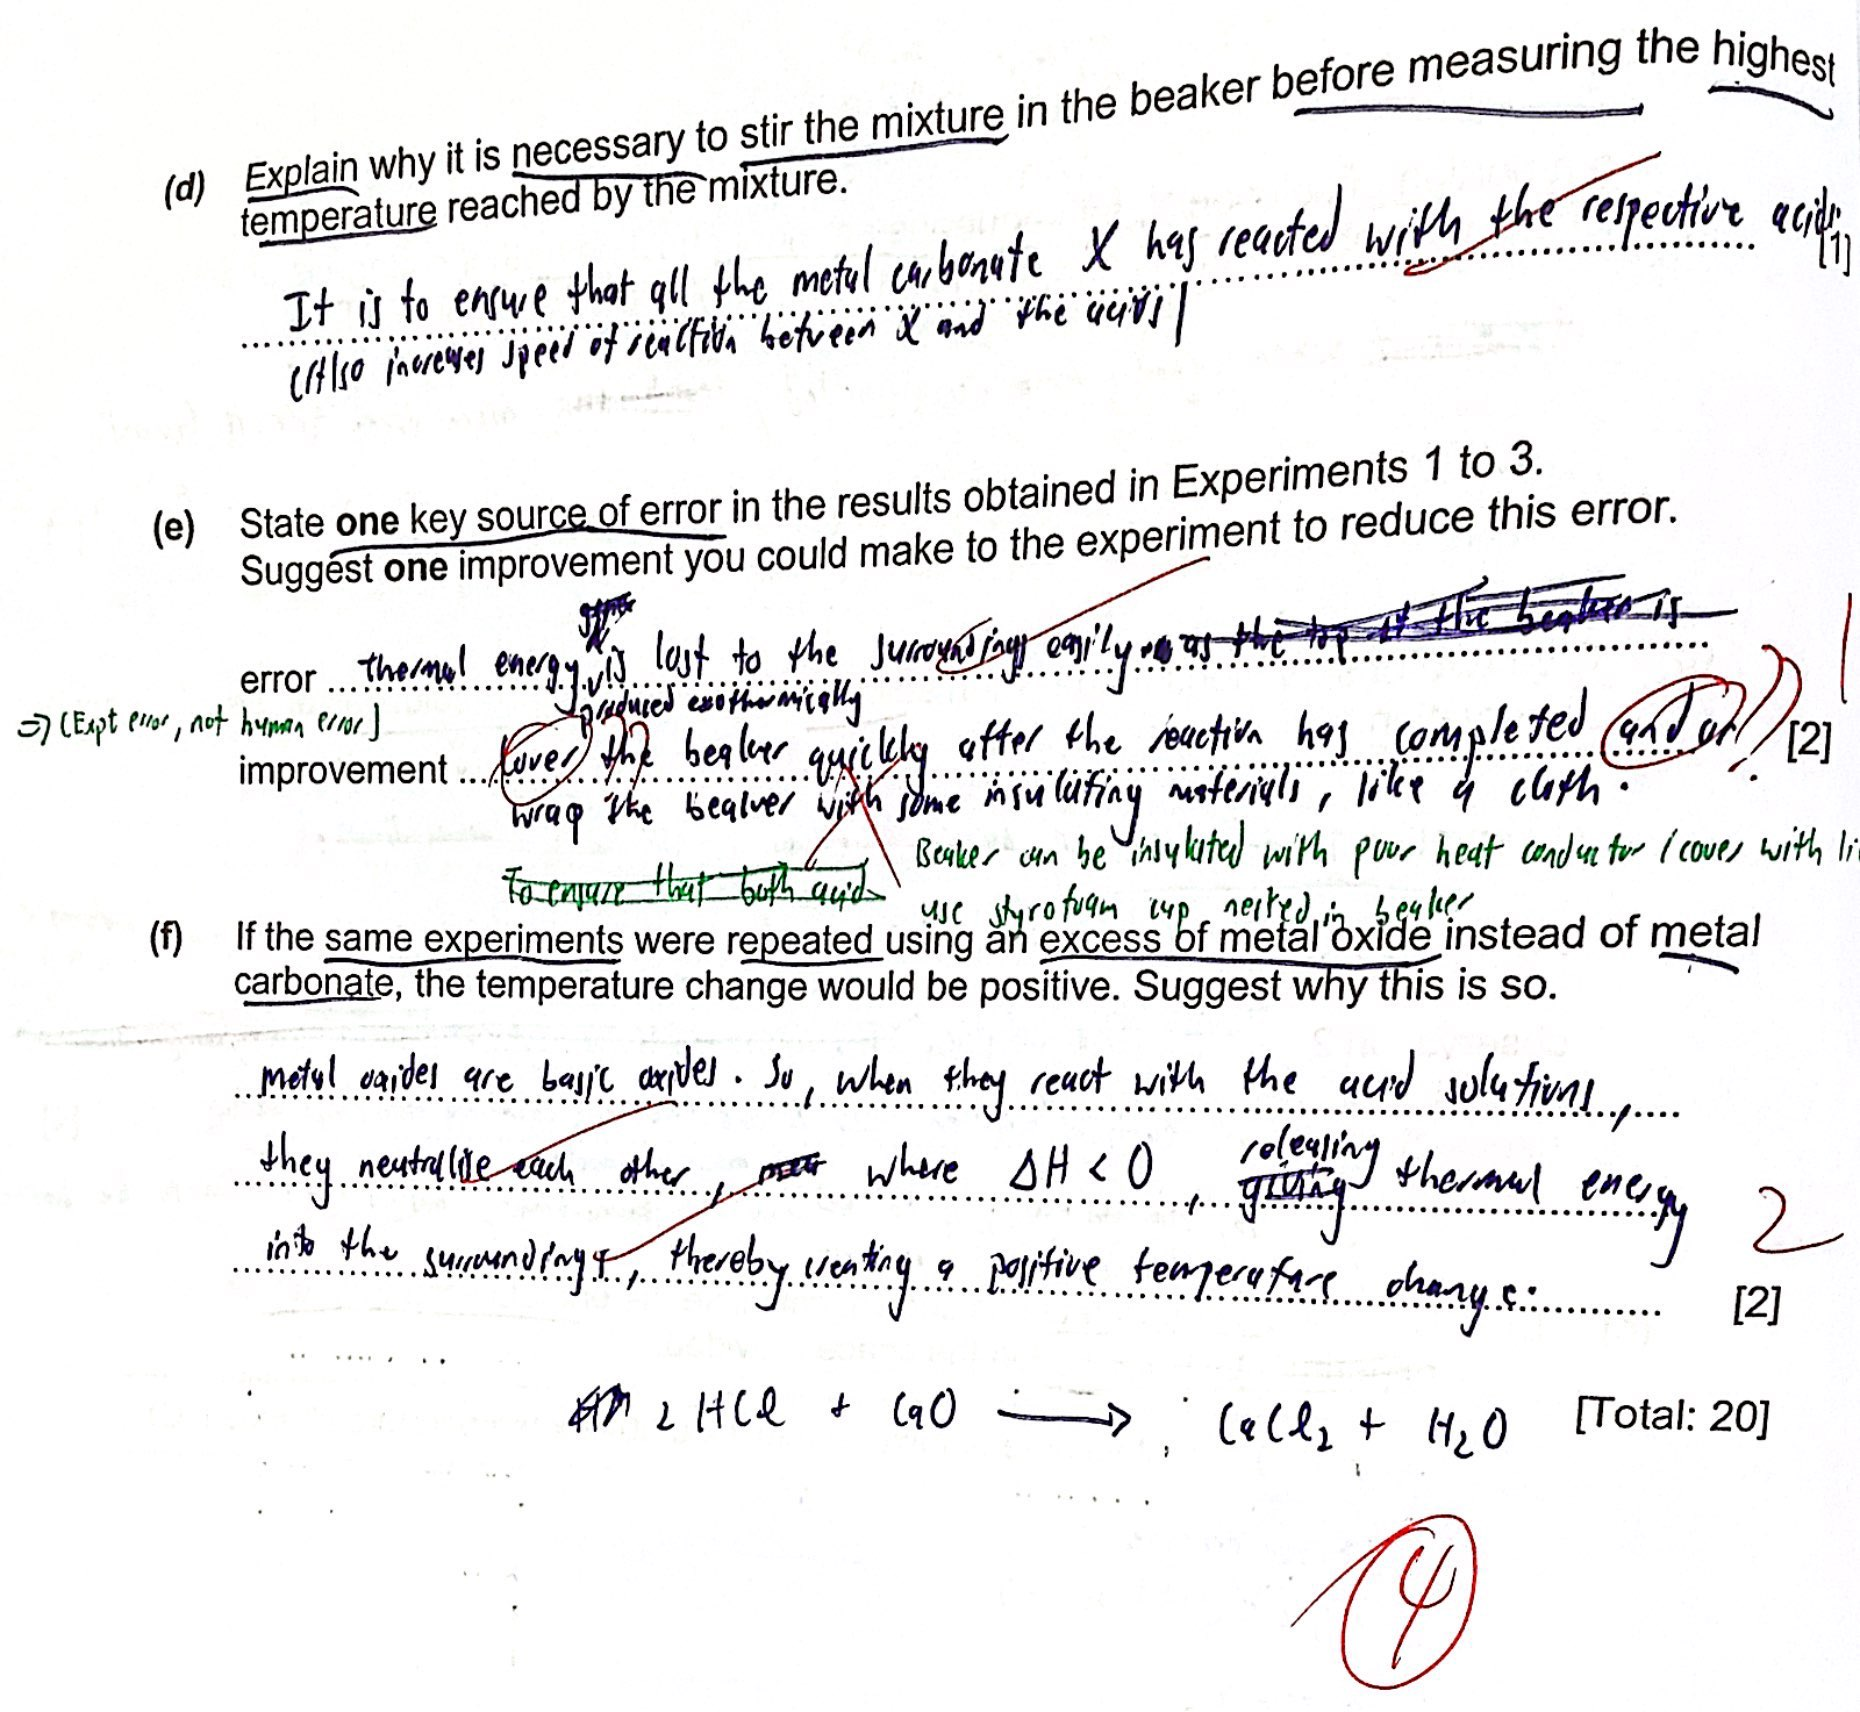
\includegraphics[width=\textwidth,height=\textheight,keepaspectratio]{images/BA119F99-18F2-4B3F-B4E9-A8EC52CEAF41.jpeg}\\
    \end{center}
    \subsection{ Combined Chemistry Q.A. Test 2020}
    \begin{center}
        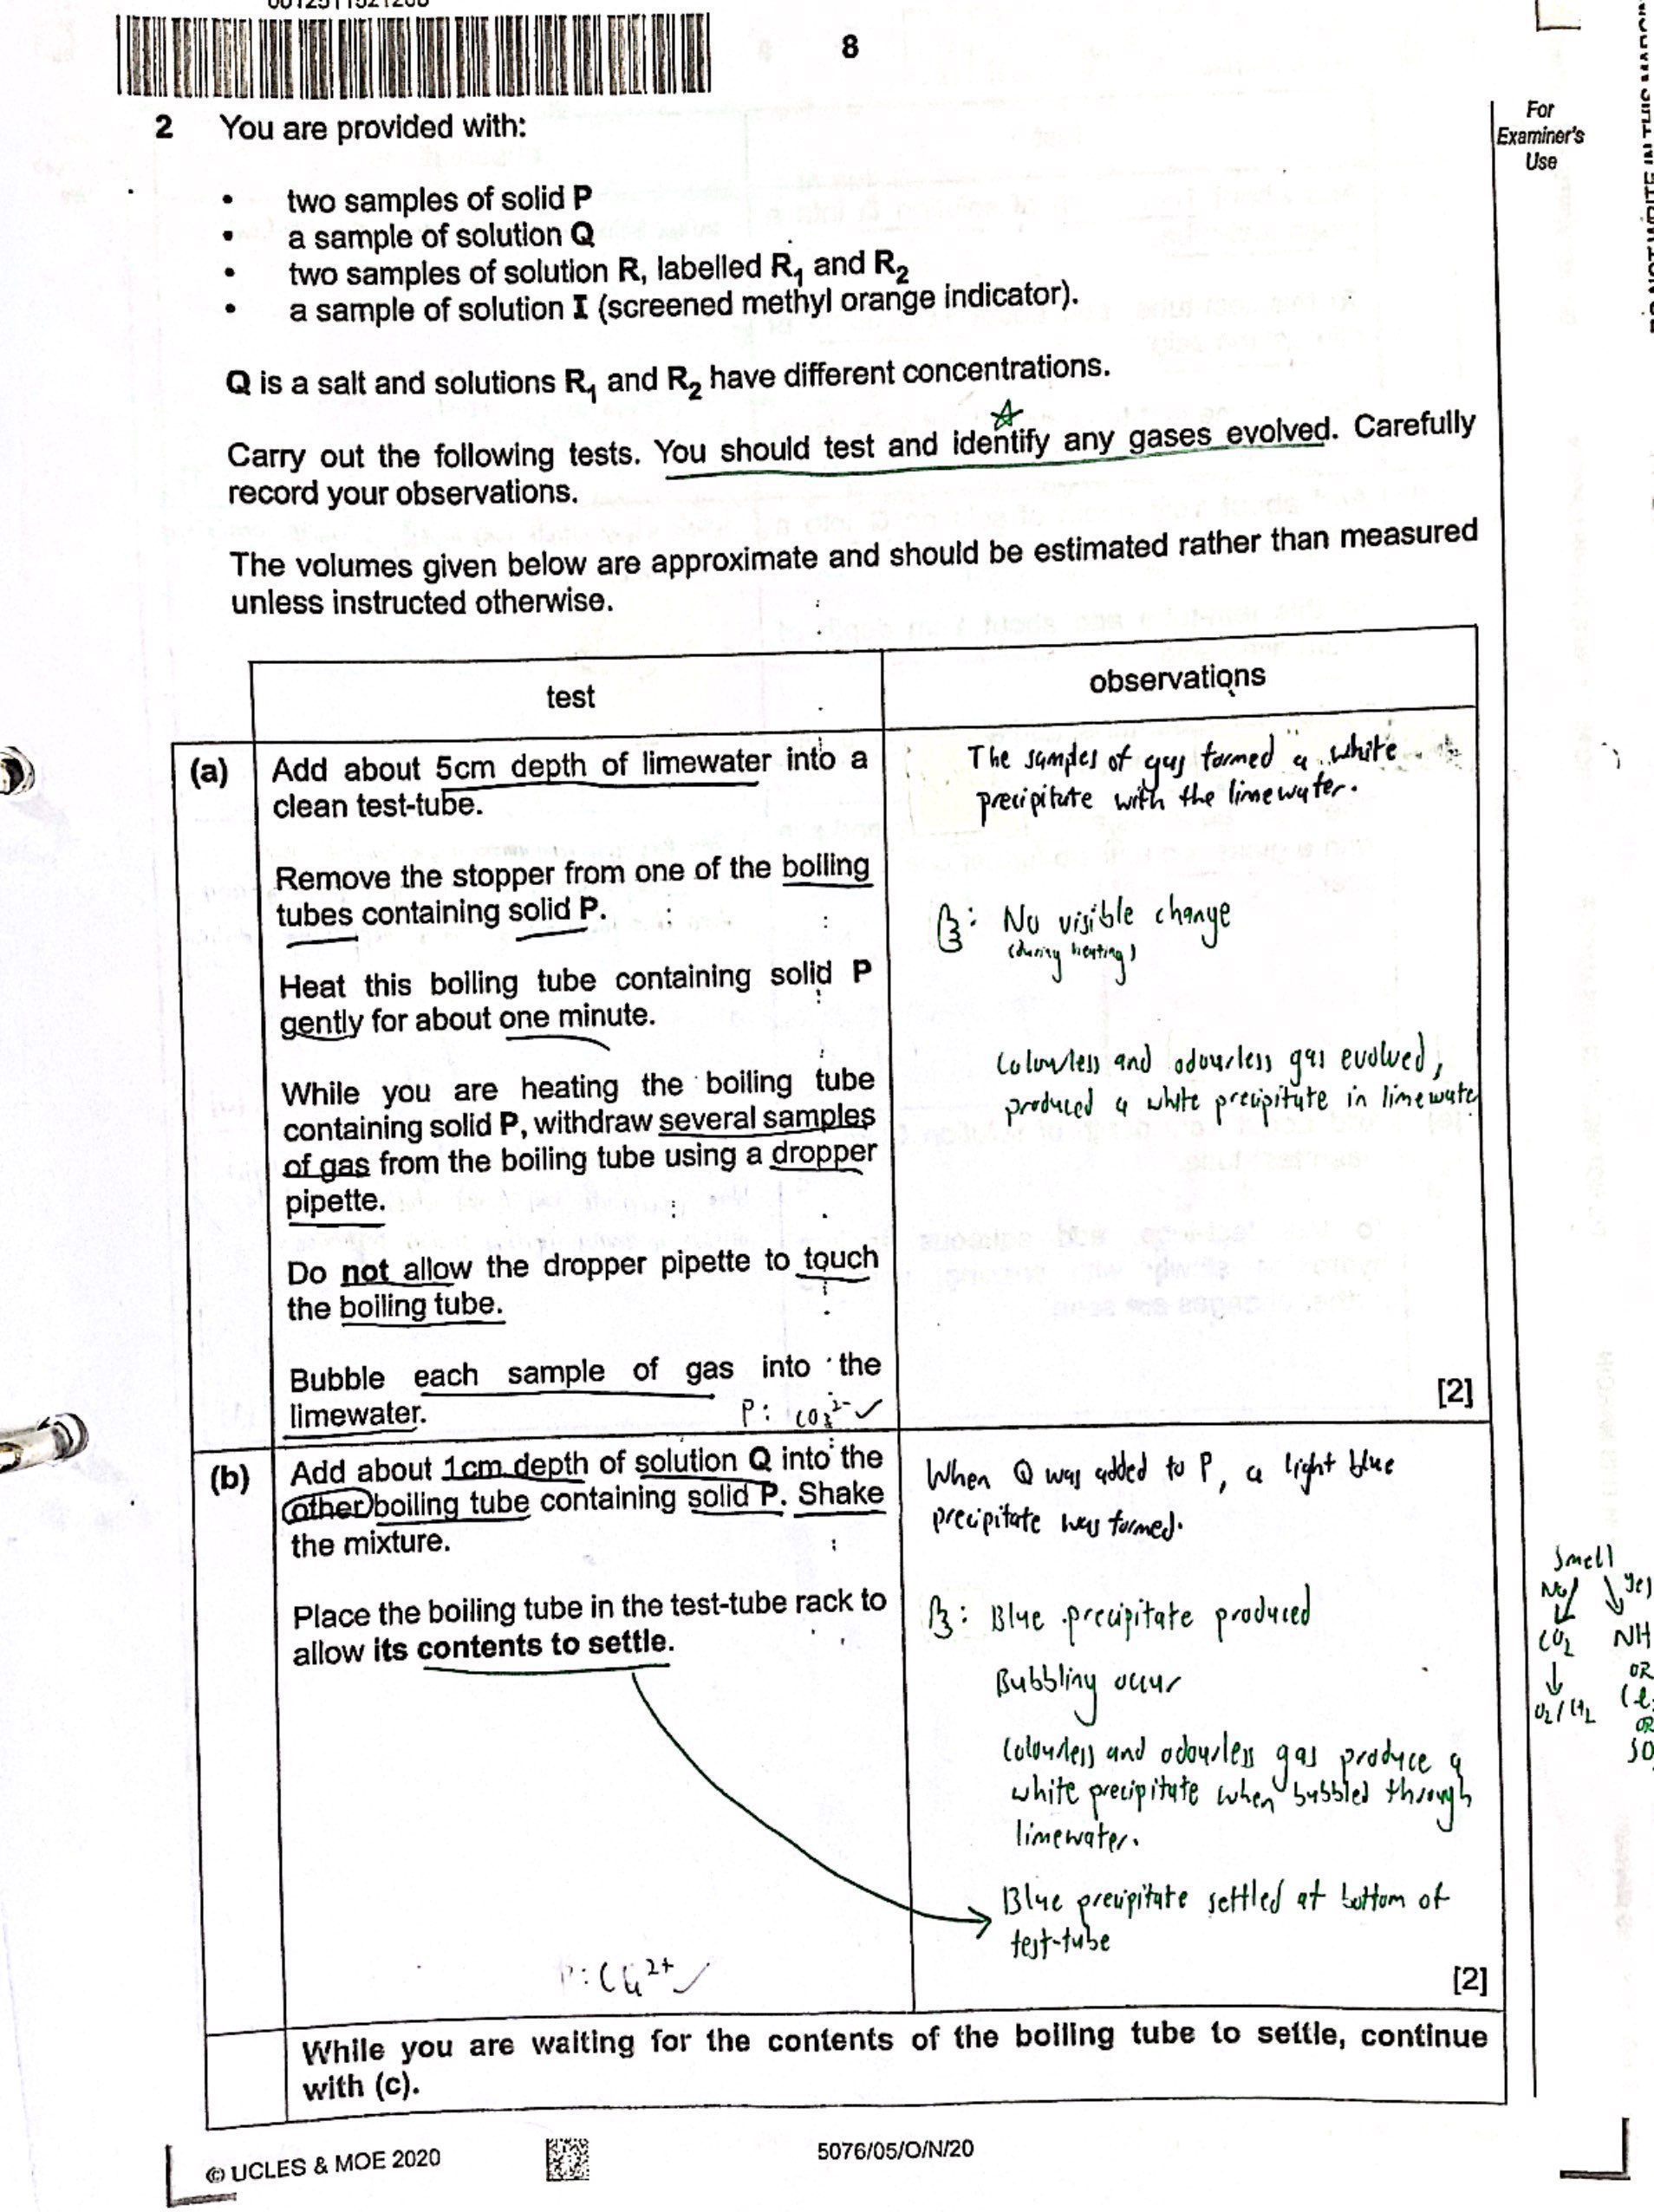
\includegraphics[width=\textwidth,height=\textheight,keepaspectratio]{images/2BDCCC19-0848-4D8E-A62C-ED809525C535.jpeg}\\
        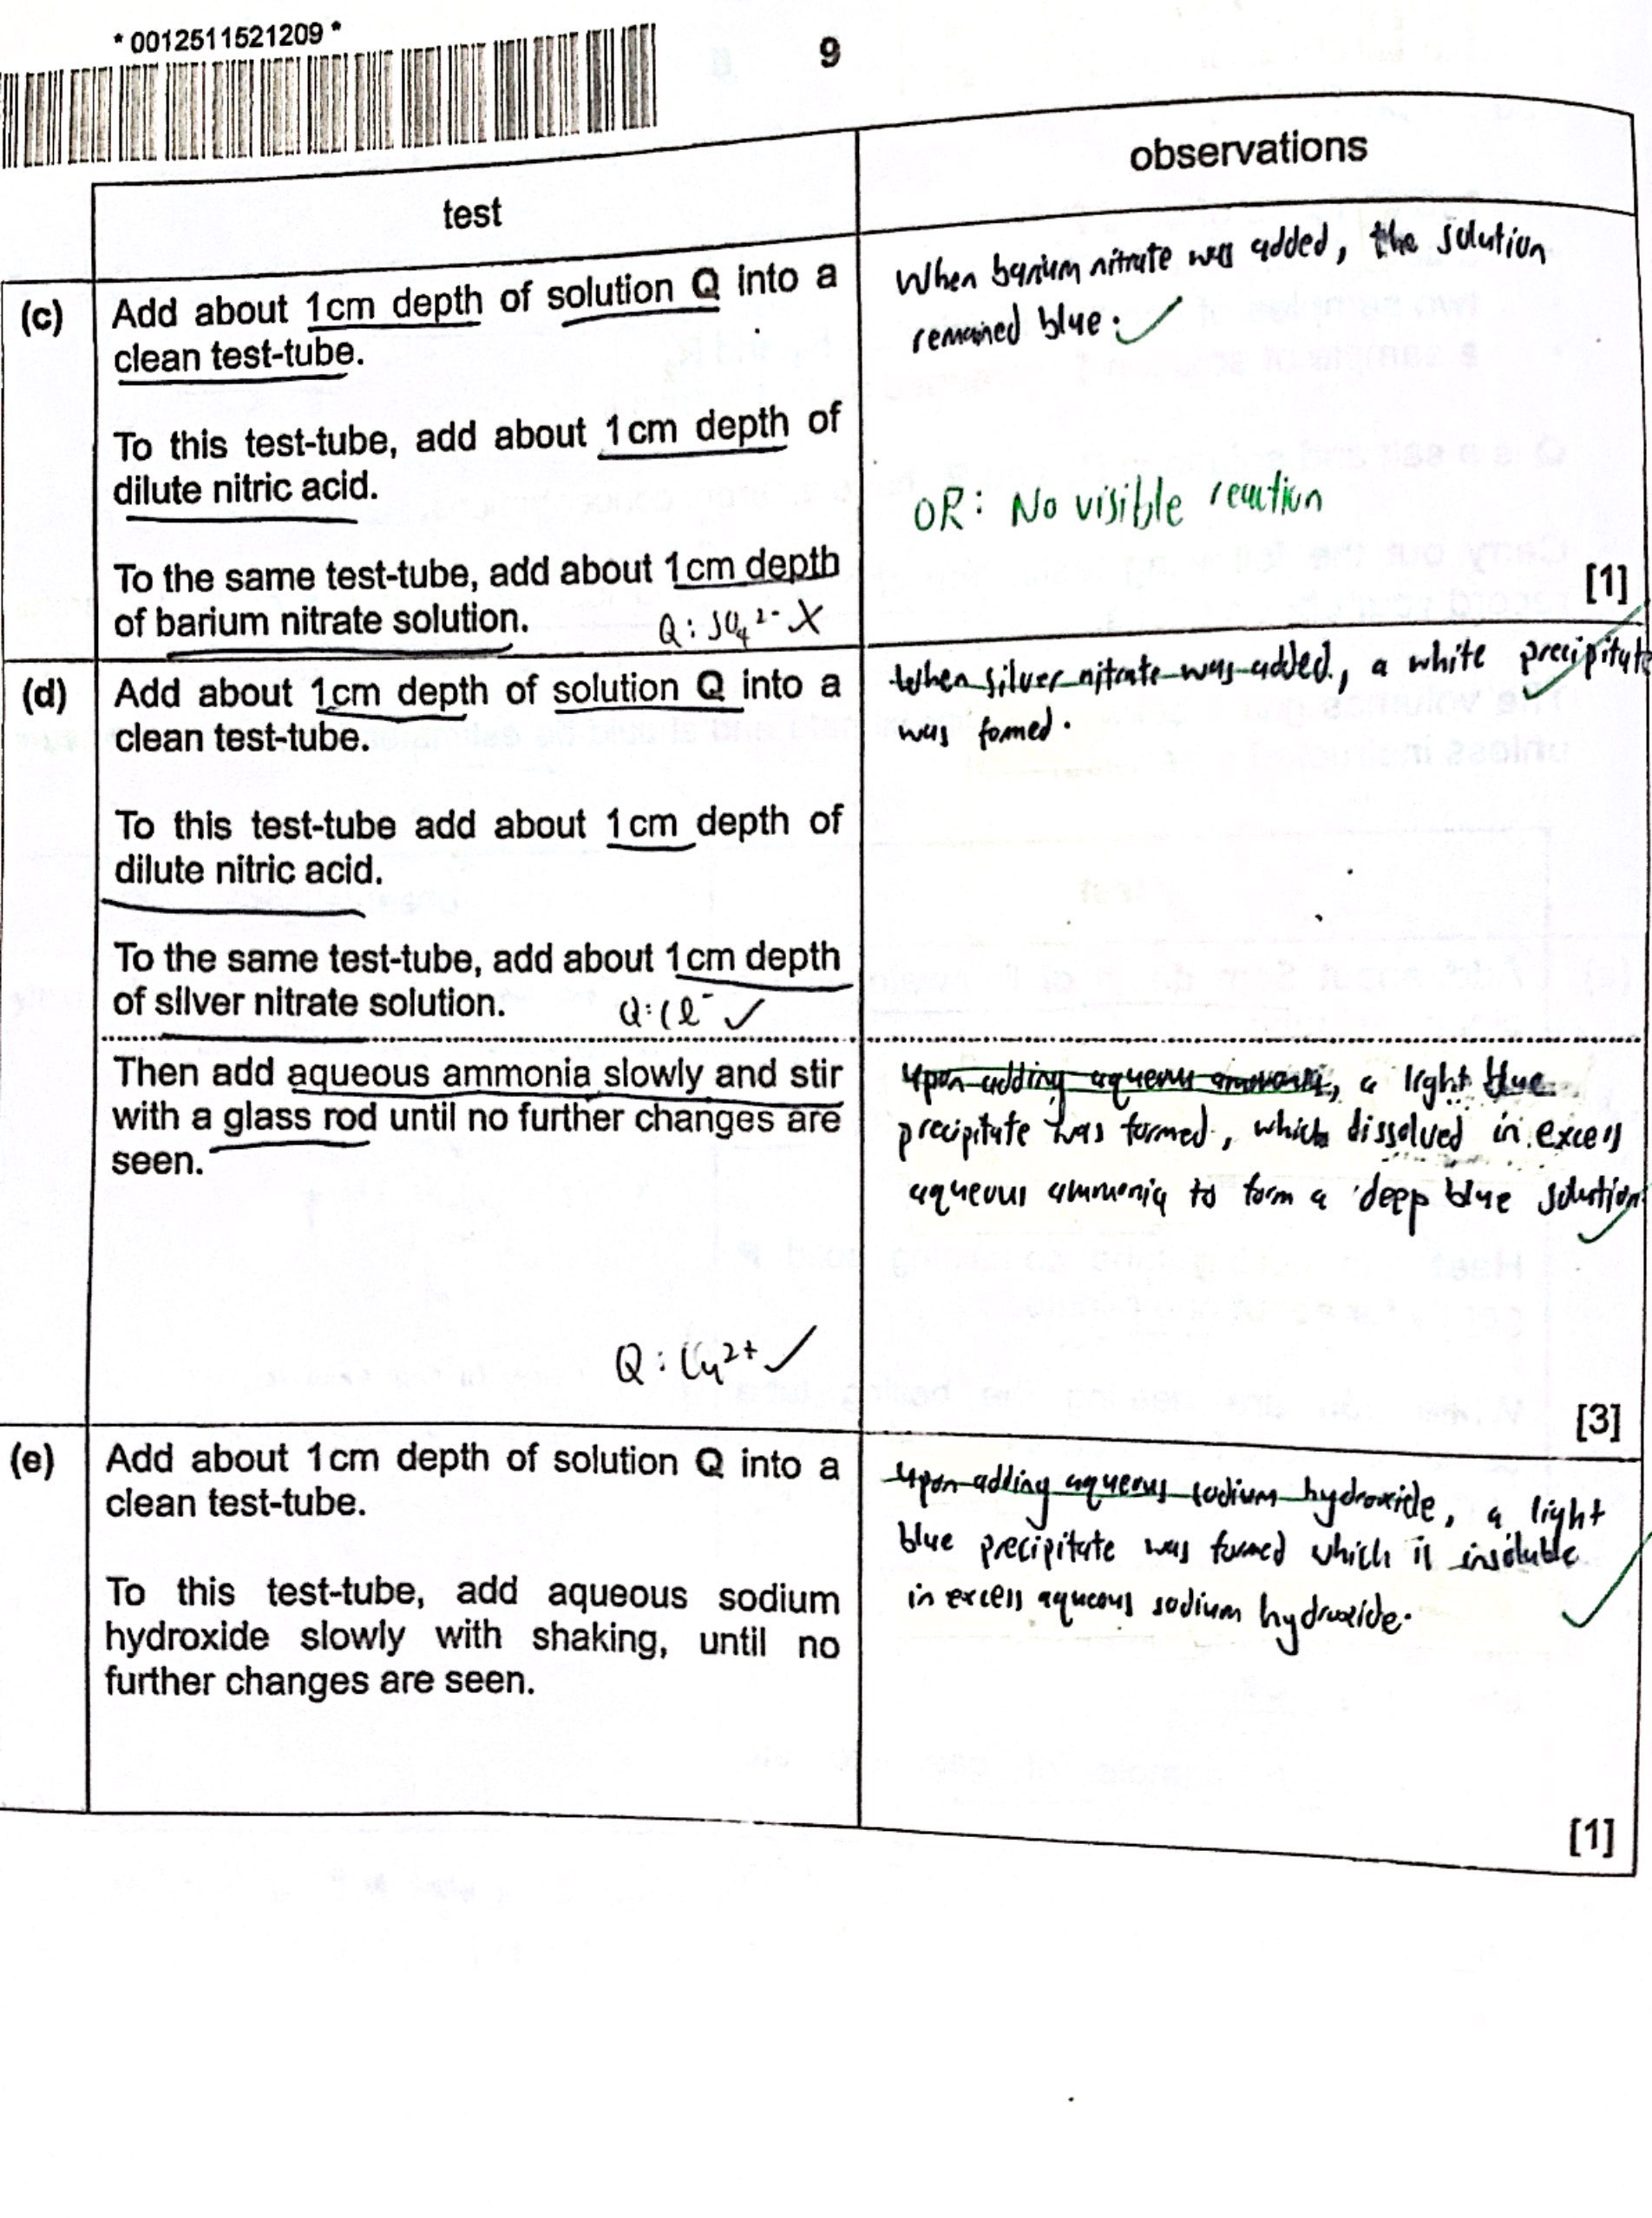
\includegraphics[width=\textwidth,height=\textheight,keepaspectratio]{images/B3CA916E-FF2B-4CE2-8230-C665B4472A20.jpeg}\\
        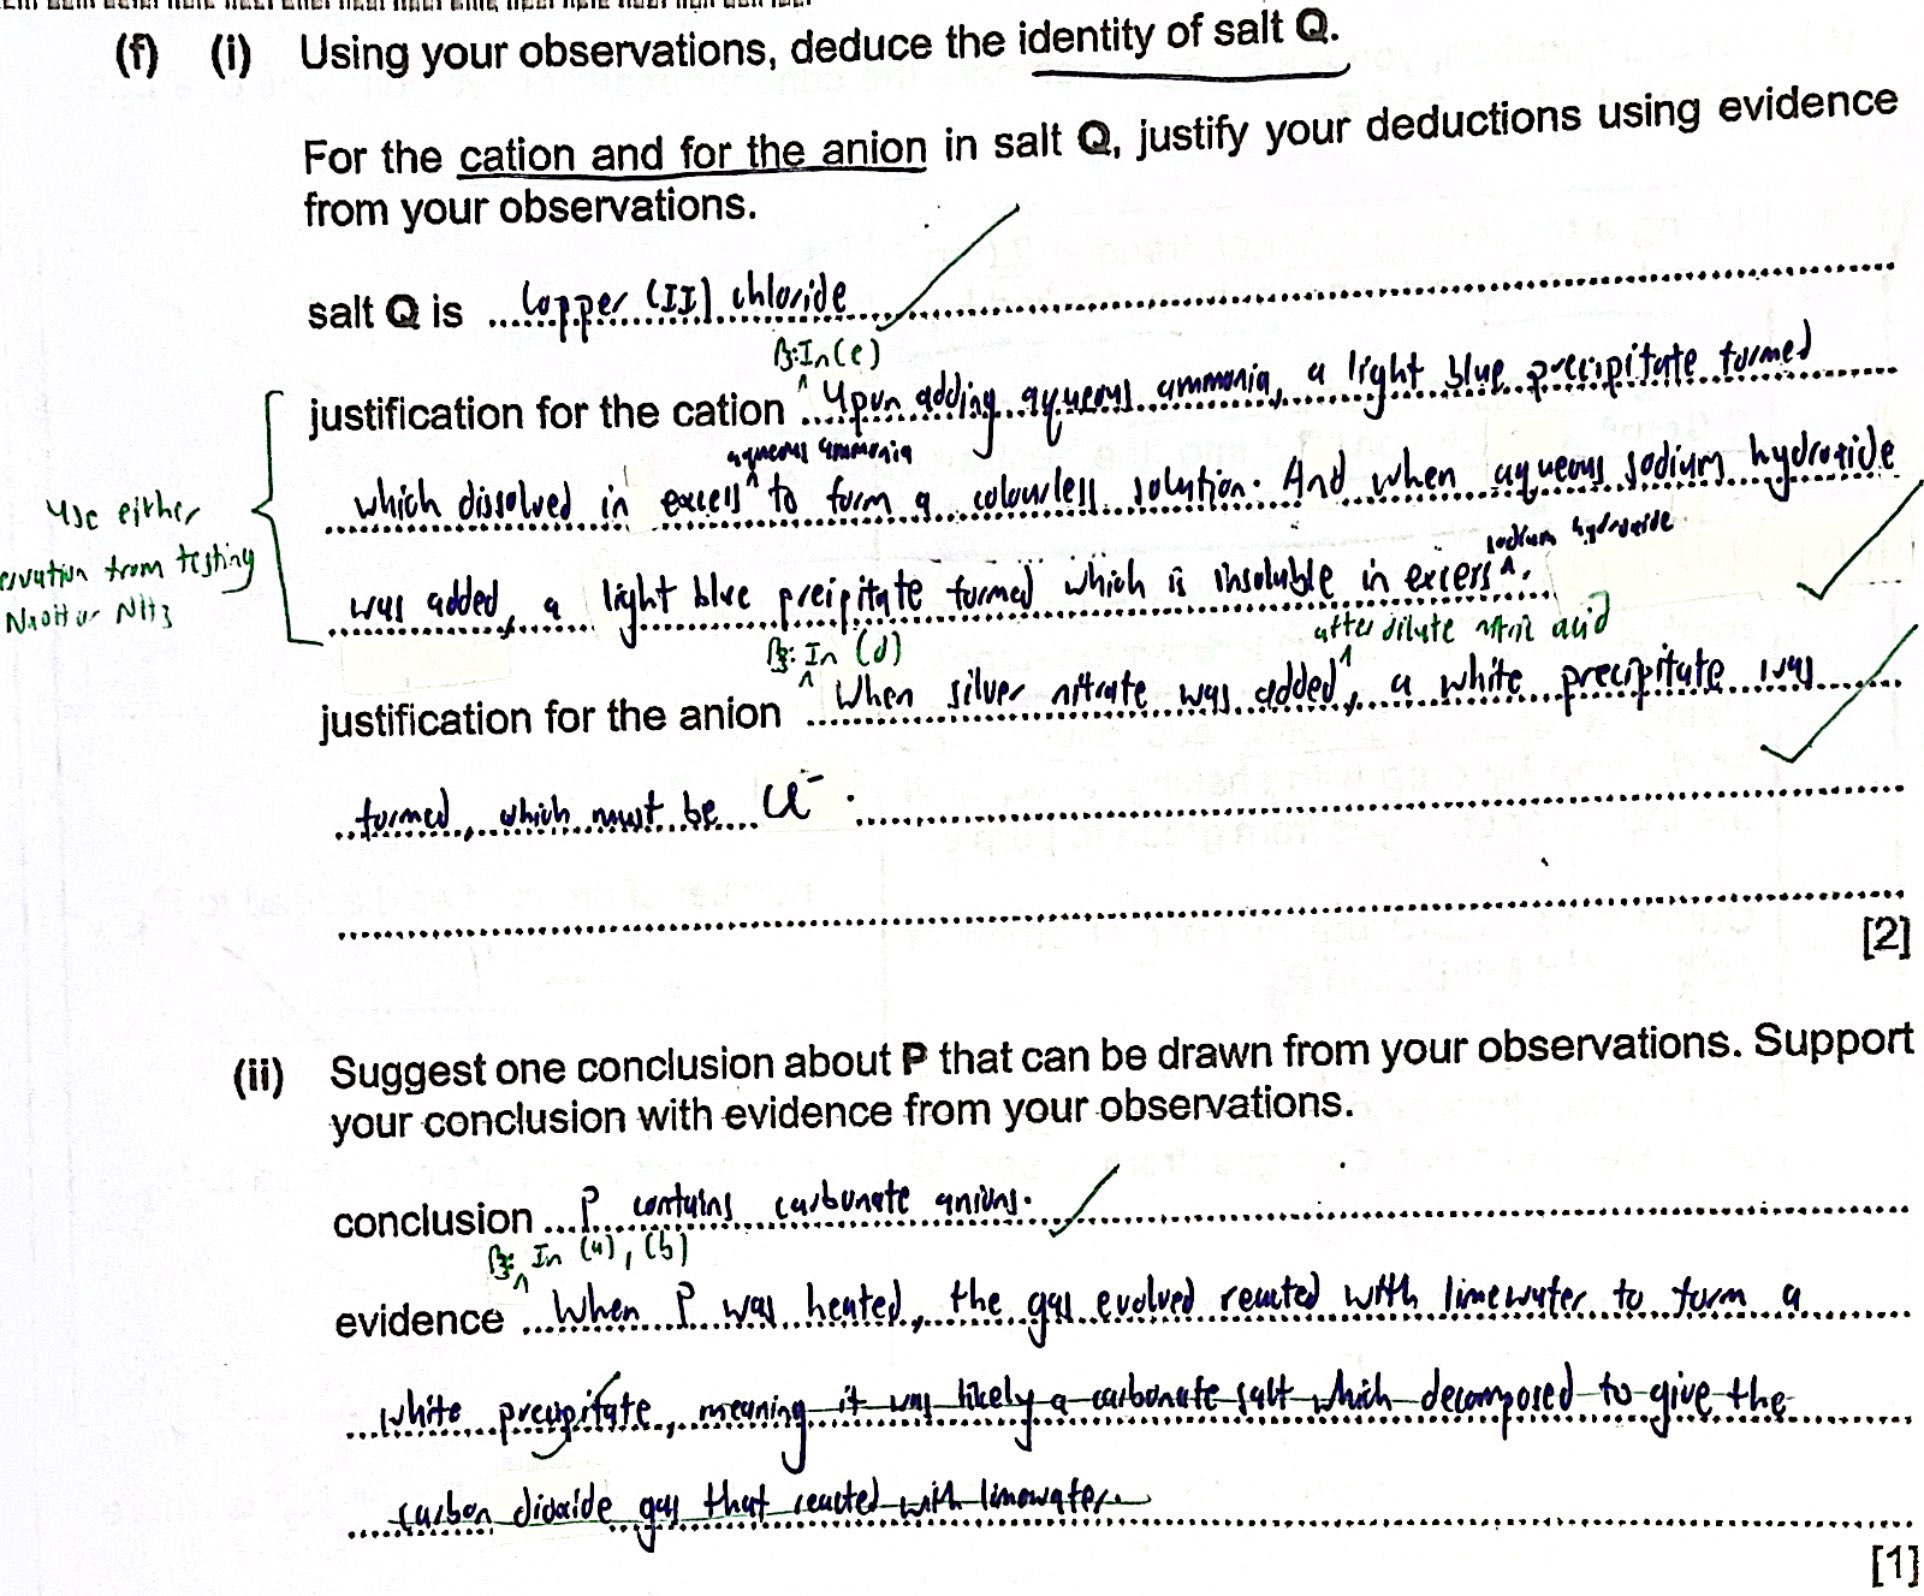
\includegraphics[width=\textwidth,height=\textheight,keepaspectratio]{images/F1A32D54-8CB3-4C0A-8D4A-AD0ACD8A5EBE.jpeg}\\
        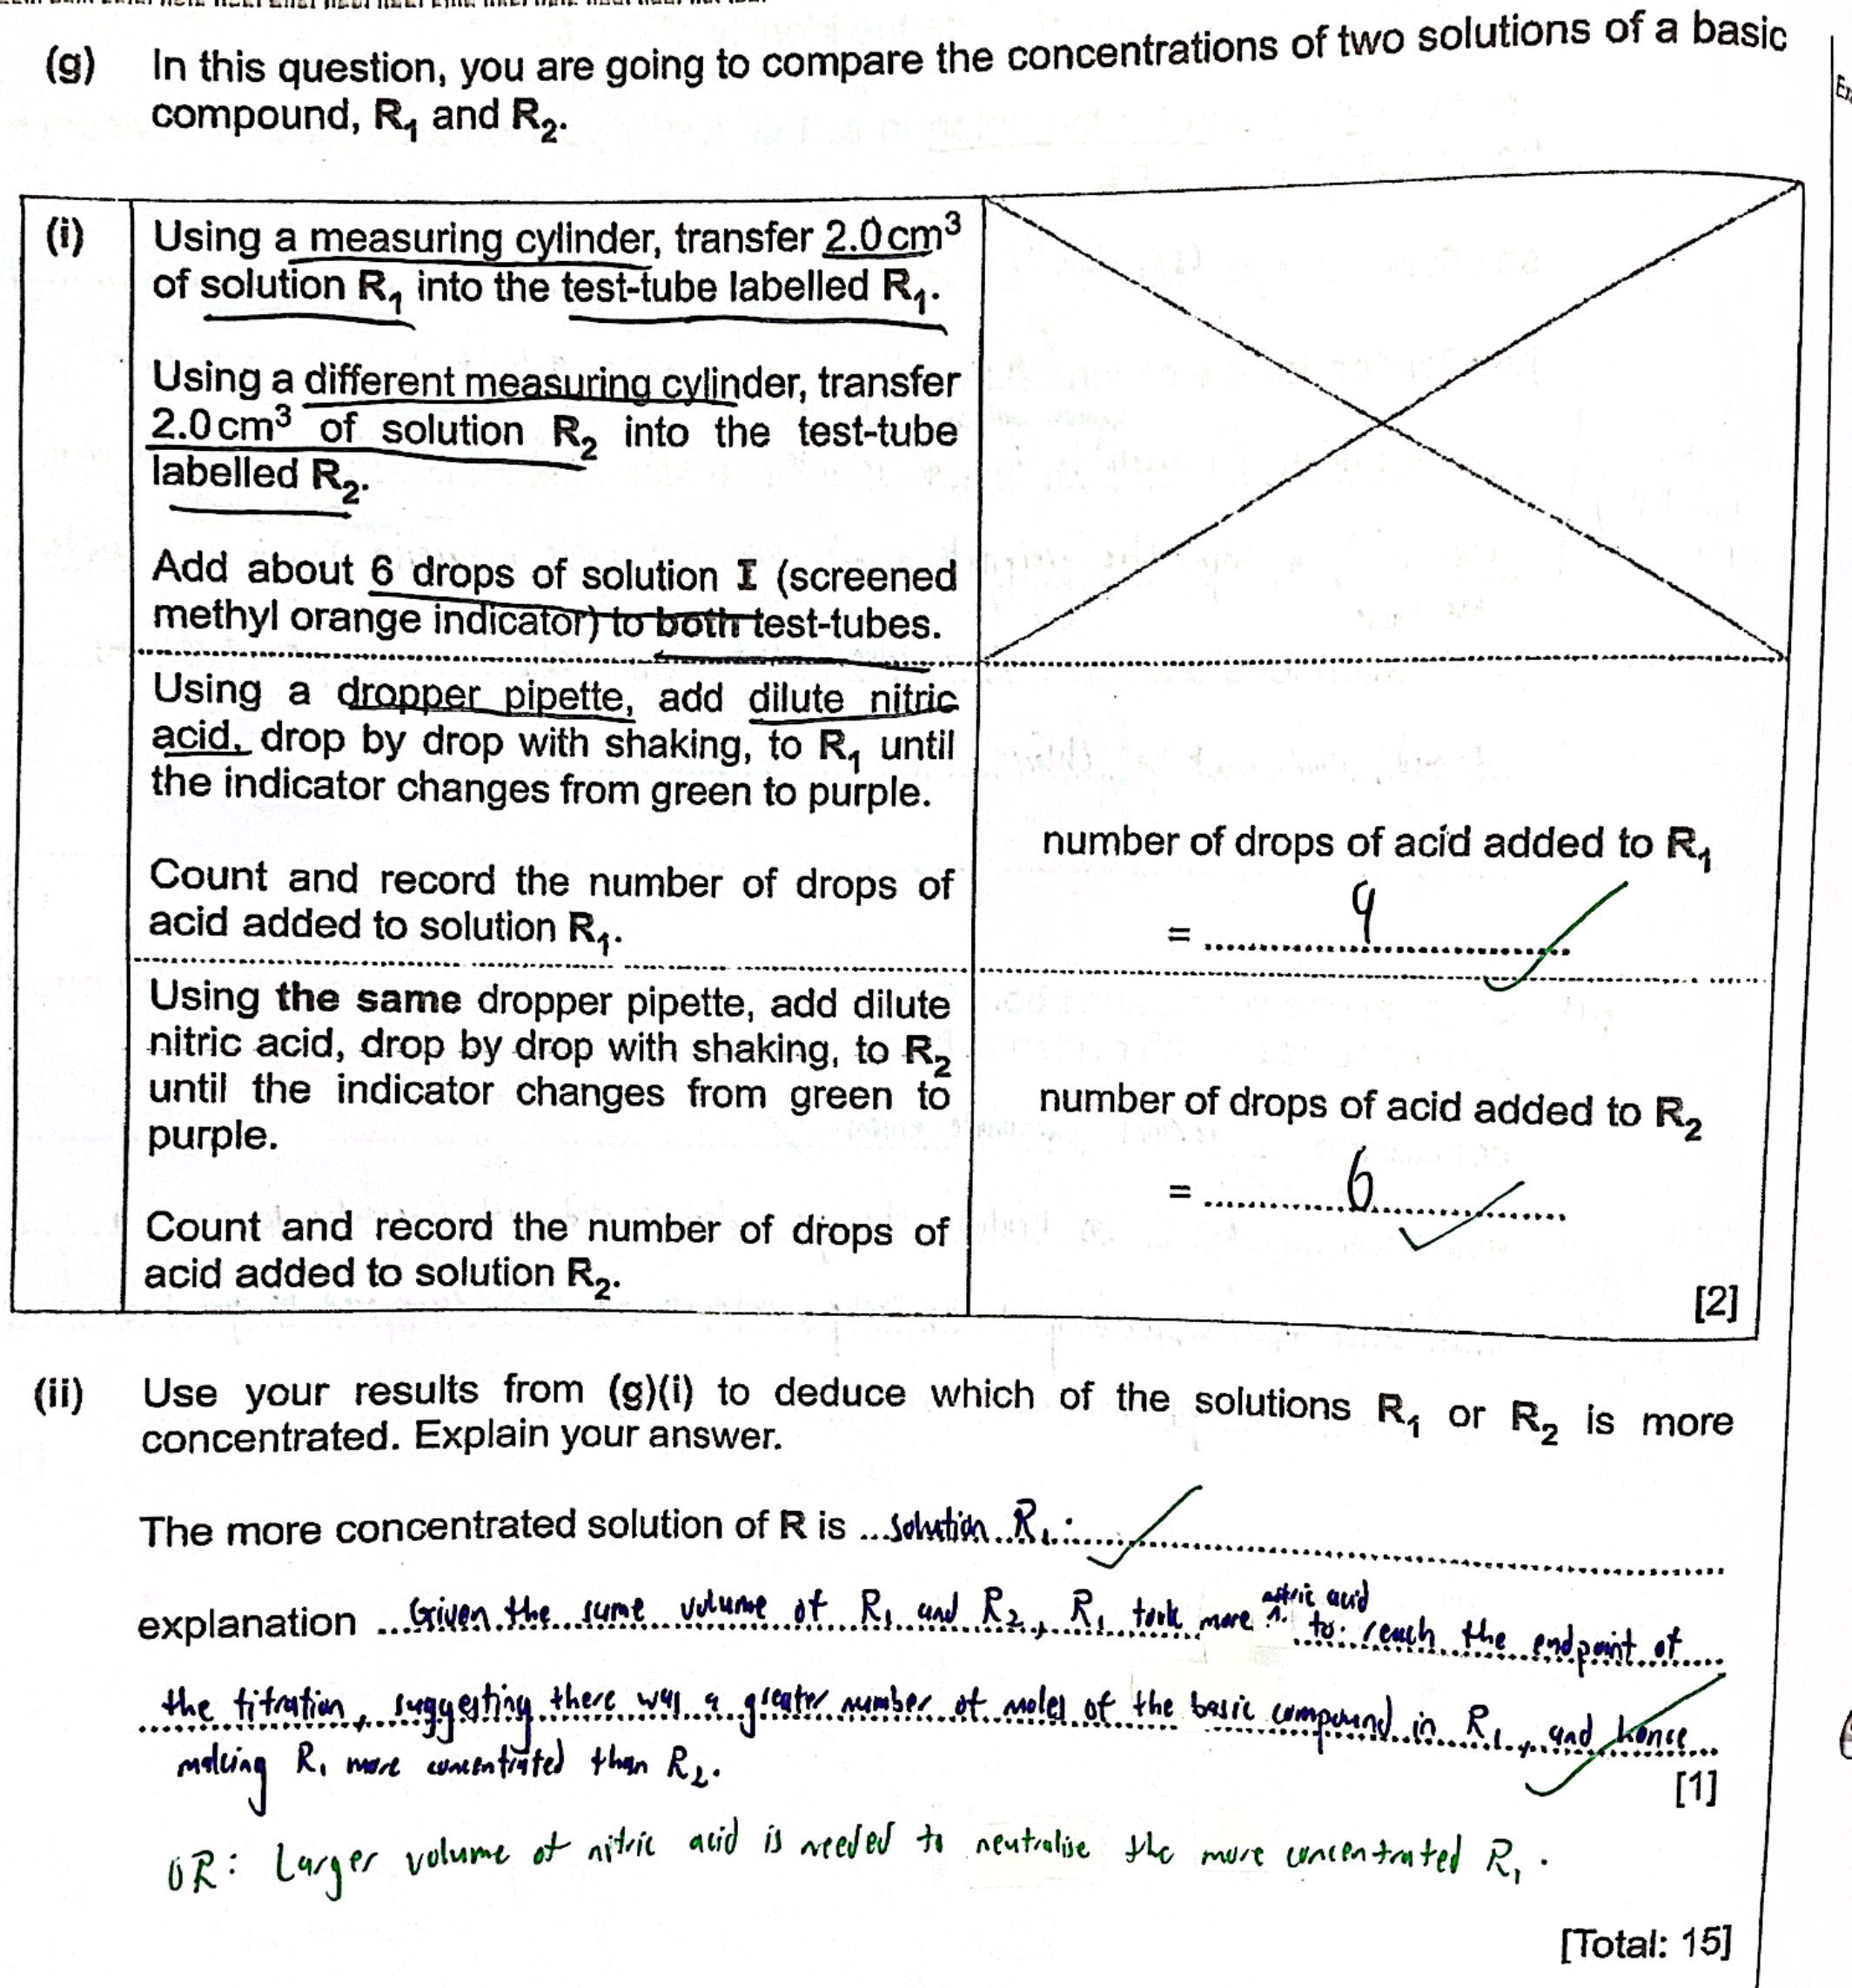
\includegraphics[width=\textwidth,height=\textheight,keepaspectratio]{images/91E14B8E-C349-48B7-9B06-51EA888F843D.jpeg}
    \end{center}
\section{Experimental Planning}
    \subsection{Timed Assignment 2022: Paper 3 Practical} \begin{center}
        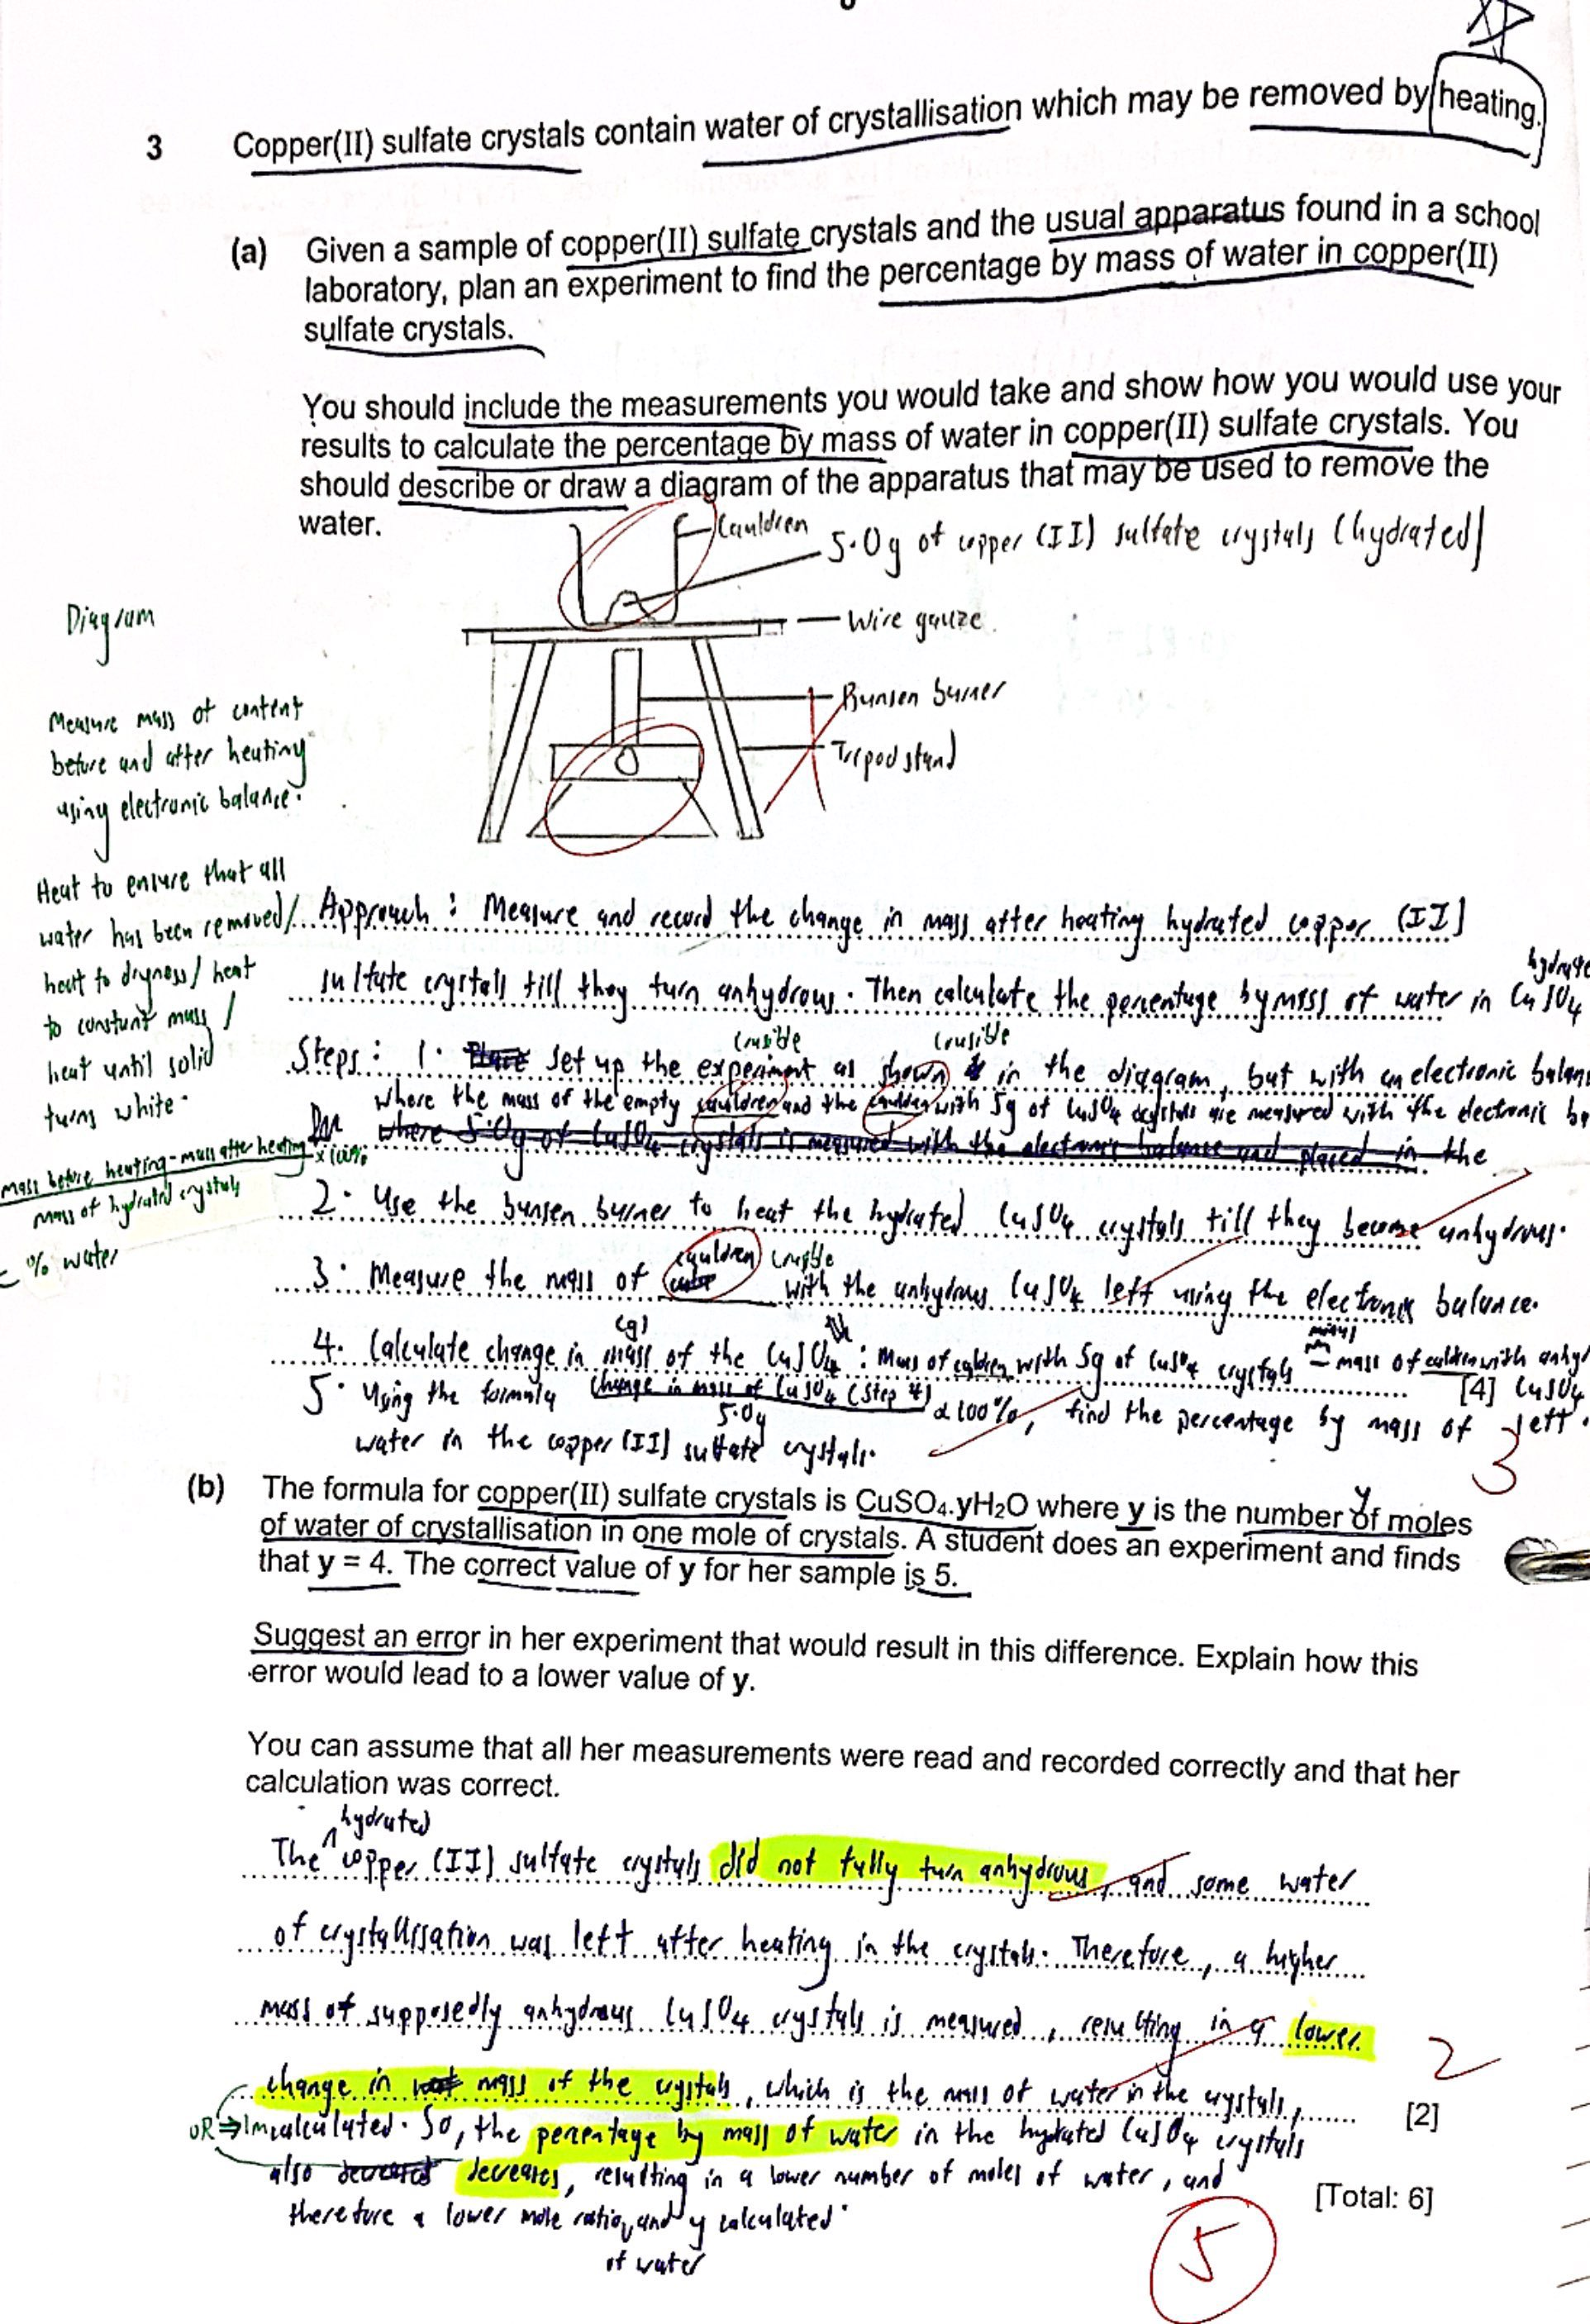
\includegraphics[width=\textwidth,height=\textheight,keepaspectratio]{images/AAC51764-8AB3-4F2E-86DA-AA8B61CADE87.jpeg}
    \end{center}
    \newpage
    \subsection{Hydrogen Peroxide decomposition, 4 April 2022}
    \begin{center}
        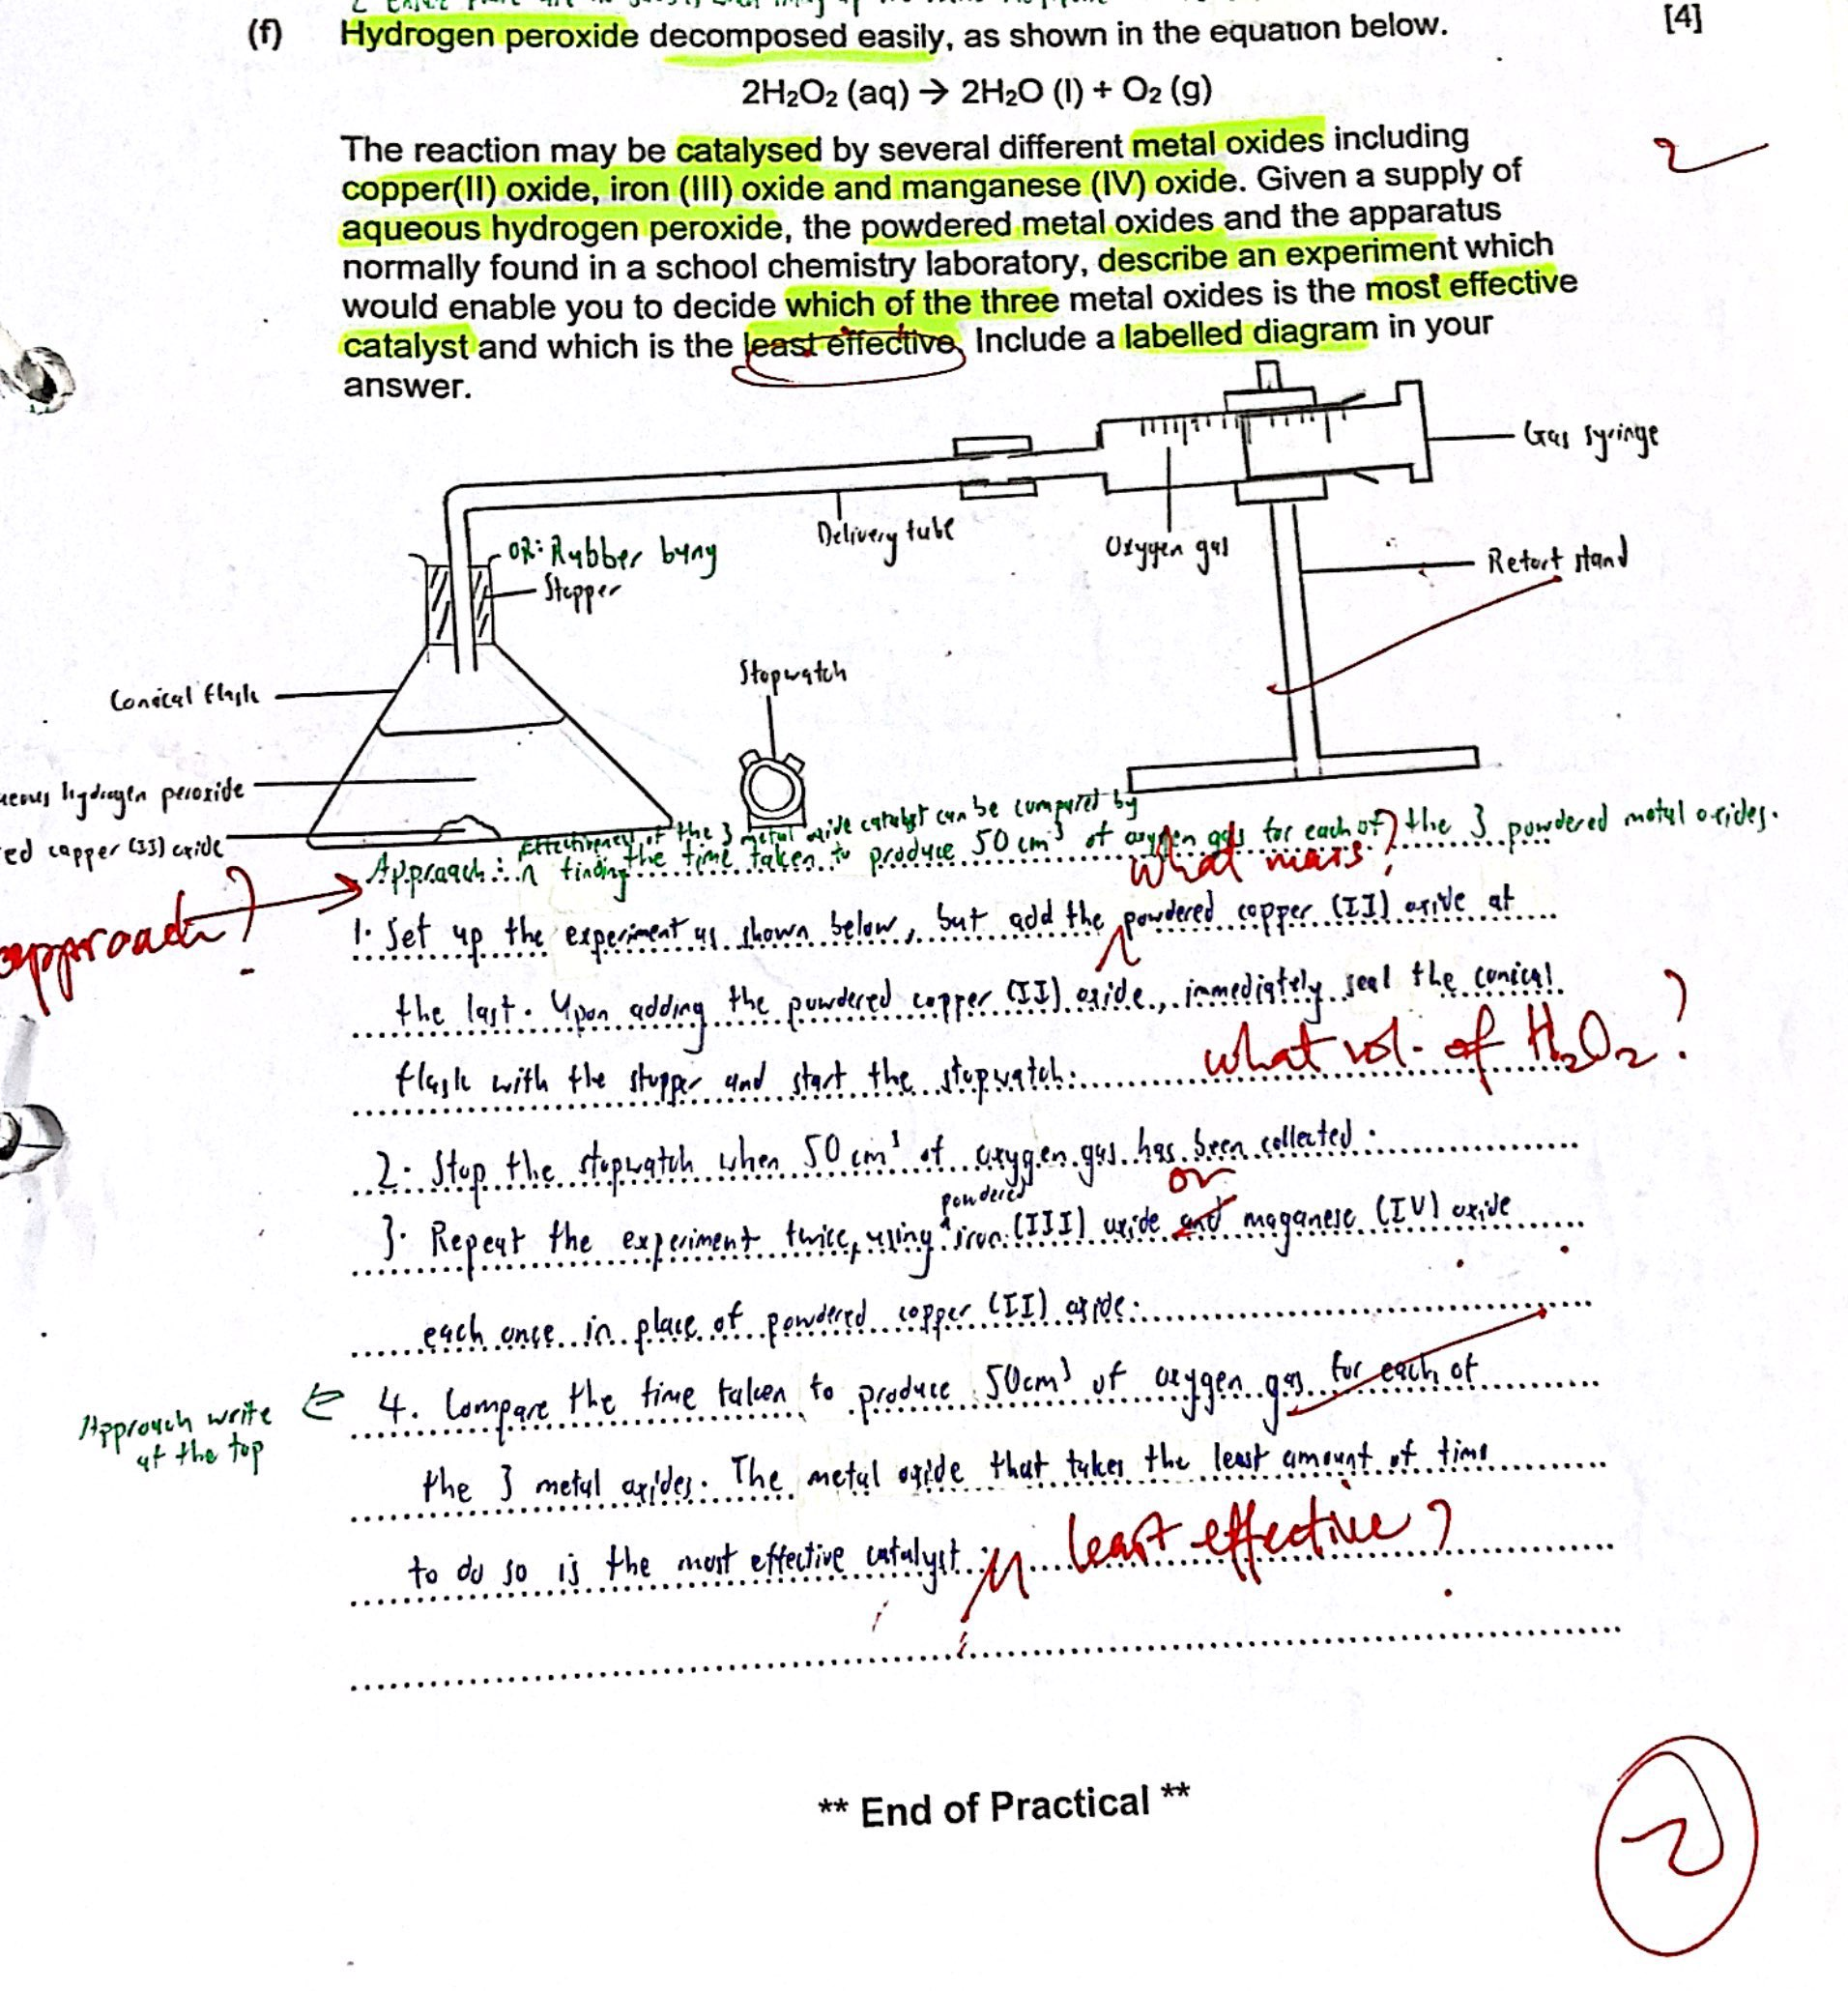
\includegraphics[width=\textwidth,height=\textheight,keepaspectratio]{images/83E95DF2-766C-402A-AF56-48AEA2066E8F.jpeg}\\
        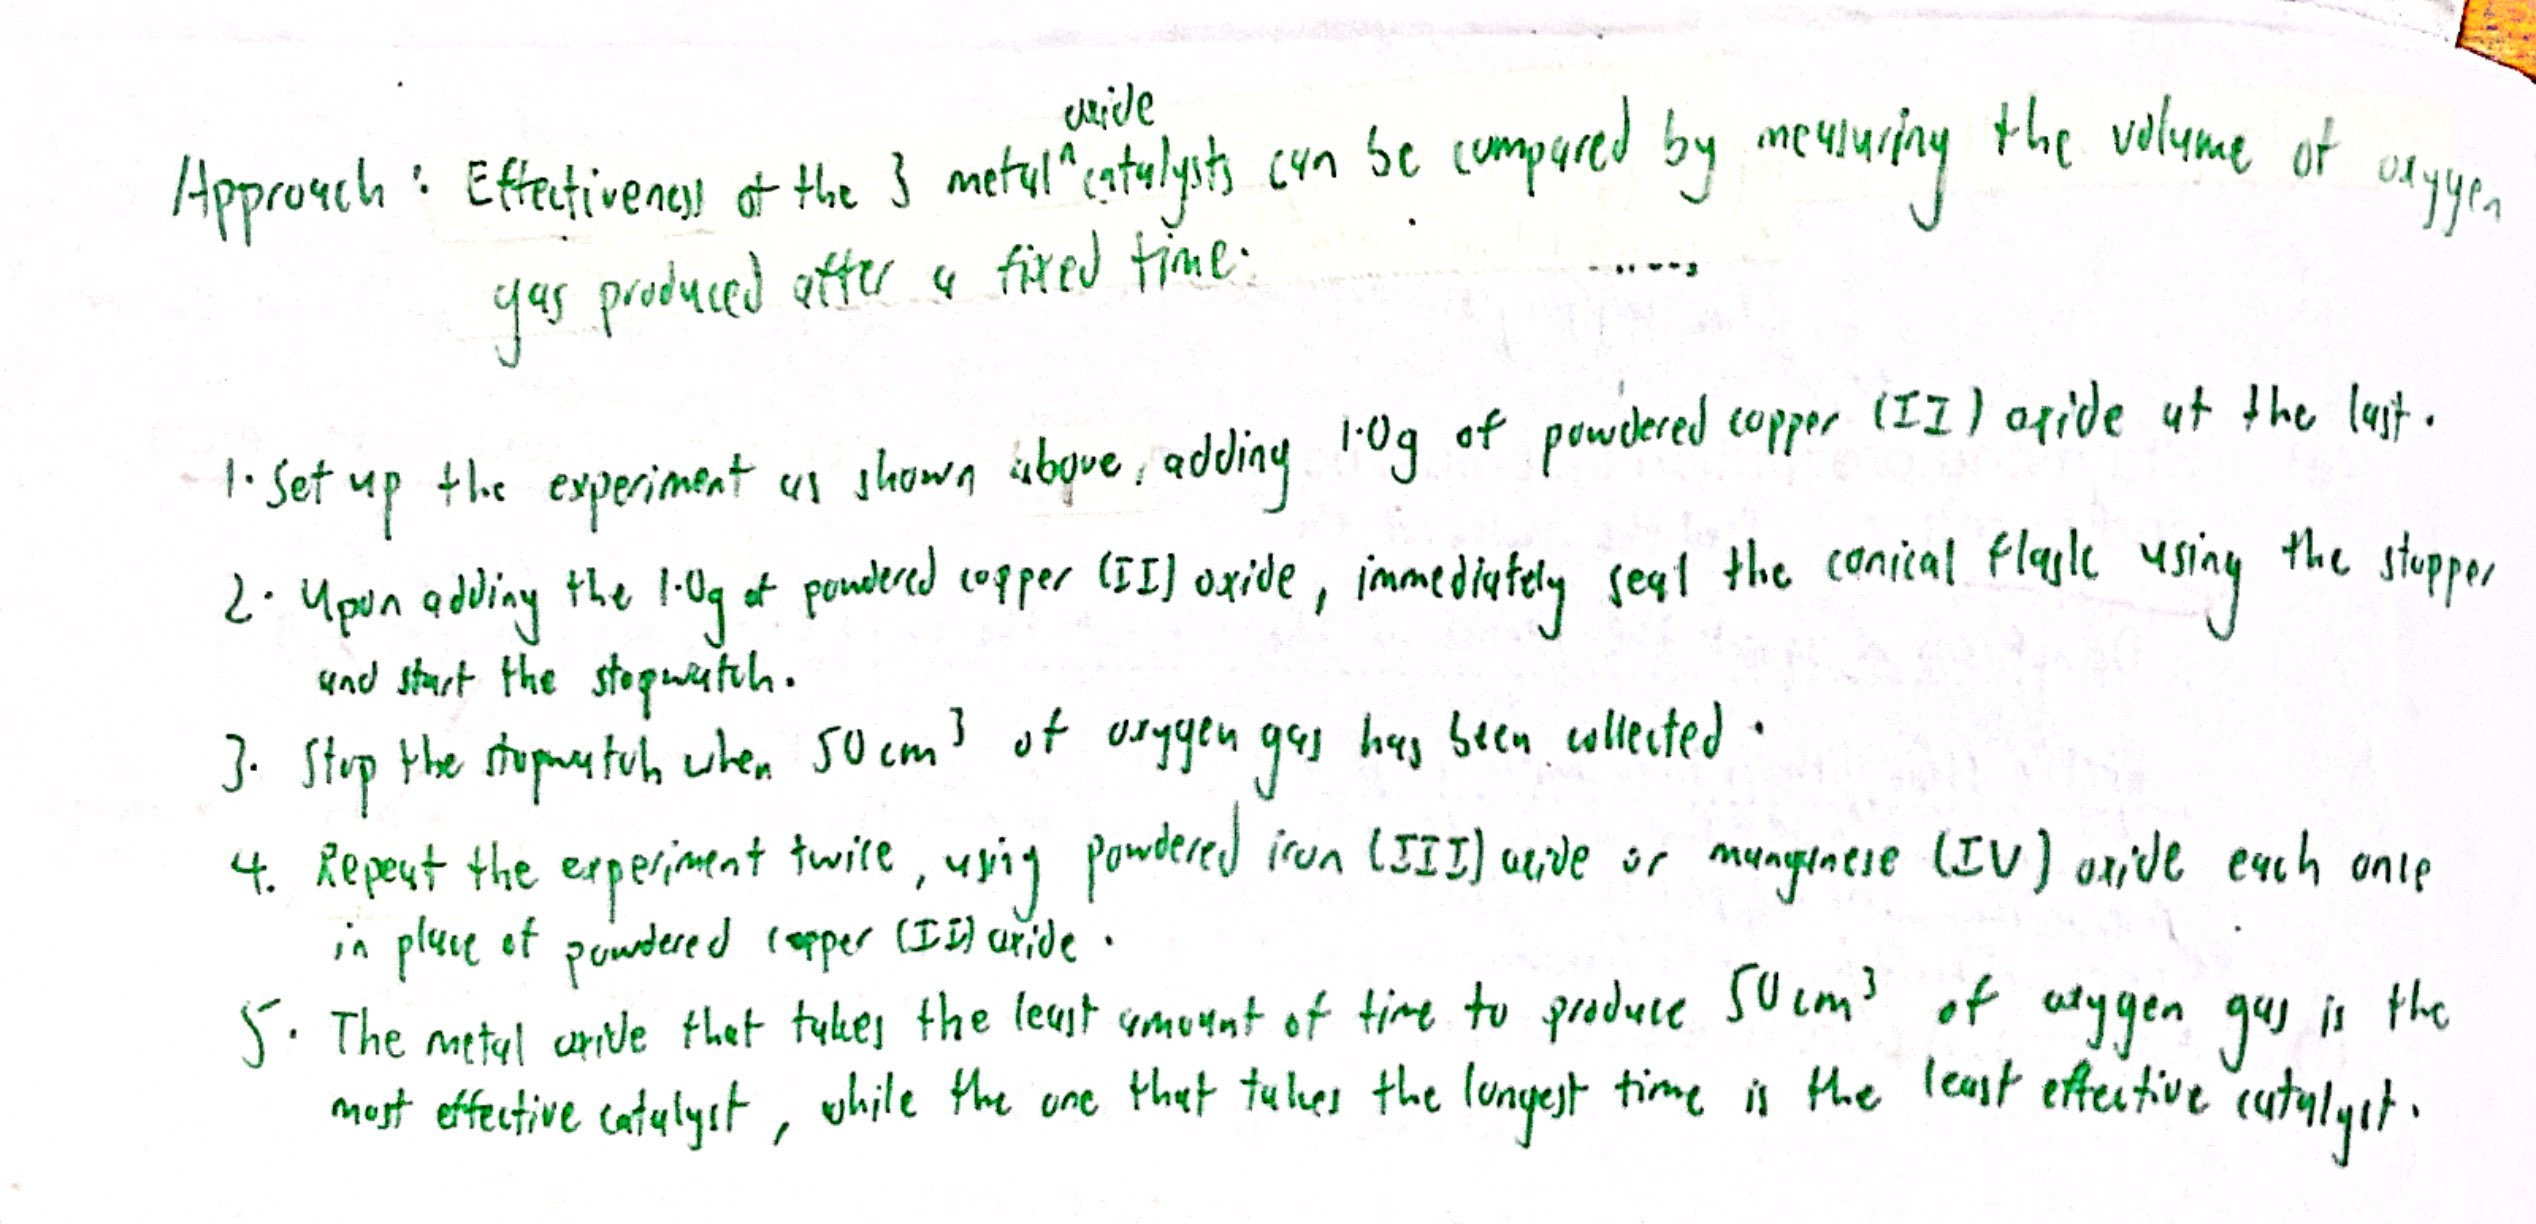
\includegraphics[width=\textwidth,height=\textheight,keepaspectratio]{images/F69305D9-6946-4FE4-BC23-FE5FBC61CF76.jpeg}
    \end{center}



\end{document}
